\chapter{Gestión del proyecto}
\label{cap:gestion}

Todo proyecto de ingeniería del software requiere, además de la resolución
técnica del problema planteado, una gestión del propio proceso de
trabajo: qué metodología se sigue, cómo se reparte el esfuerzo en el tiempo,
qué recursos se necesitan y qué riesgos pueden comprometer el resultado
final. Este capítulo documenta esa gestión para el presente proyecto: la
metodología de trabajo adoptada, las fases en que se ha dividido el
desarrollo, los roles ejercidos, la planificación temporal (inicial y
revisada), la estimación de recursos y presupuesto, y los planes de gestión
de riesgos y de calidad aplicados.

\section{Metodología de trabajo}
\label{sec:gestion-metodologia}

Este proyecto se ha desarrollado siguiendo un enfoque iterativo e
incremental, guiado por instrucciones de seguimiento con el tutor.
En lugar de fijar de antemano una especificación cerrada de todo el sistema
, cada bloque de trabajo se ha
planteado como una iteración corta que produce un resultado funcional y
evaluable, cuyas conclusiones determinan el siguiente paso. Este enfoque es
especialmente adecuado en un proyecto como este,
en el que algunas decisiones como qué algoritmos comparar, qué metadatos
extraer, hasta dónde llevar la calibración de cámara dependían de
resultados intermedios que no podían conocerse de antemano: no tenía
sentido, por ejemplo, comprometerse a un pipeline completo de metadatos
antes de comprobar que la comparativa de algoritmos de tracking daba
resultados sólidos y defendibles.

Dentro de ese marco iterativo, cada ciclo de trabajo ha seguido
aproximadamente la misma secuencia: (1) plantear una pregunta concreta o un
objetivo acotado a partir de las conclusiones del ciclo anterior y, en las
ideas claves de las instrucciones del tutor; (2) implementar la
solución mínima que permita responder a esa pregunta; (3) evaluar el
resultado con datos reales, normalmente mediante las métricas MOT estándar
descritas en el capítulo~\ref{cap:fundamentos}; y (4) plantear la idea y 
decisiones tomadas al tutor y documentar la decisión
tomada (incluida la opción de descartar el enfoque probado) antes de
pasar al siguiente ciclo. Este último punto ha sido determinante para la
redacción de esta memoria: al quedar registrada la razón de cada decisión
en el momento en que se tomó, ha sido posible construir la memoria de forma
detallada, incluyendo no solo los resultados finales, sino también el proceso seguido para llegar hasta ellos.

El seguimiento del trabajo entre reuniones se ha apoyado en un documento de
anotaciones propio, actualizado de forma continua, donde se registran
decisiones tomadas, resultados numéricos, problemas de entorno encontrados
y su solución, e ideas evaluadas y descartadas. Este documento ha sido la fuente principal para poder
documentar todo el proceso de desarrollo en esta memoria.

\section{Fases del proyecto}
\label{sec:gestion-fases}

Sobre la metodología iterativa descrita, el trabajo se ha organizado en
siete fases principales, que se recorrieron de forma mayoritariamente
secuencial pero con solapamientos puntuales entre fases adyacentes; en
particular entre la fase 4 (estudio de hiperparámetros) y la fase 5
(pipeline de metadatos), ya que la configuración óptima de cada algoritmo
se fue consolidando mientras ya se trabajaba en los primeros metadatos, y
entre la fase 5 y la fase 7 (redacción de la memoria), que se ha llevado en
paralelo a las últimas iteraciones técnicas en lugar de posponerse por
completo al final del proyecto.

La primera fase correspondió a la exploración de las distintas tareas que
ofrece el ecosistema SoccerNet antes de comprometerse con ninguna de ellas,
descrita con más detalle en la sección~\ref{sec:analisis-decision} del
capítulo~\ref{cap:analisis}. Una vez elegido el tracking como tarea del
proyecto, las fases 2 y 3 cubrieron la implementación de los dos algoritmos
comparados y su evaluación con métricas estándar, primero sobre el
conjunto de entrenamiento y, a petición del tutor, también sobre el
conjunto de test. Las fases 4 y 5 constituyen el núcleo experimental del
proyecto: el estudio sistemático de hiperparámetros y el diseño del
pipeline de extracción de metadatos deportivos sobre la configuración
óptima resultante. La fase 6, desarrollo de la aplicación web, se completó
como un MVP fiel al diseño planificado en el capítulo~\ref{cap:diseno},
según se detalla en la sección~\ref{subsec:gestion-revision}. La
Tabla~\ref{tab:gestion-fases} resume estas siete fases, sus actividades
principales y el resultado obtenido en cada una.

\begin{table}[htp]
\centering
\caption{Resumen de las fases del proyecto.}
\label{tab:gestion-fases}
\renewcommand{\arraystretch}{1.3}
\begin{tabular}{|p{2.9cm}|p{5.2cm}|p{5.4cm}|}
\hline
\rowcolor{gray!25}
\textbf{Fase del proyecto} & \textbf{Actividades principales} & \textbf{Resultado obtenido} \\
\hline
1. Exploración inicial &
  Estudio de diferentes tareas alternativas de SoccerNet (reconocimiento de dorsales,
  segmentación de cámara, tracking) y primeras pruebas de visualización sobre
  el \emph{ground truth} &
  Elección de la tarea (tracking) y del enfoque de asociación sobre
  detecciones precomputadas \\
\hline
2. Implementación de trackers &
  ByteTrack y OC-SORT con \texttt{boxmot}, filtrado geométrico del balón,
  ejecución sobre el conjunto de entrenamiento &
  Resultados de tracking para las 57 secuencias de train \\
\hline
3. Evaluación &
  Integración de TrackEval, cálculo de HOTA/MOTA/IDF1 sobre train y,
  posteriormente, sobre test &
  Comparativa inicial ByteTrack vs.\ OC-SORT \\
\hline
4. Estudio de hiperparámetros &
  Barrido uno a uno de los parámetros de cada algoritmo sobre test &
  Configuración óptima de ByteTrack y de OC-SORT \\
\hline
5. Pipeline de metadatos &
  Clasificación de equipos, mapas de calor, homografía (distancia/velocidad),
  posesión de balón &
  Metadatos deportivos extraídos sobre la configuración óptima \\
\hline
6. Aplicación web &
  Desarrollo de una interfaz de demostración y análisis de datos &
  MVP funcional \\
\hline
7. Redacción de la memoria &
  Documentación de todo el proceso, en paralelo a las últimas iteraciones
  técnicas &
  Este documento \\
\hline
\end{tabular}
\end{table}

\section{Roles y participantes}
\label{sec:gestion-roles}

El proyecto ha sido realizado por una única persona, Carlos, que ha
asumido de forma sucesiva los distintos roles que en un
contexto profesional de mayor envergadura recaerían en perfiles y personas
distintas. Definir estos roles explícitamente, aunque el proyecto sea
individual, tiene dos utilidades prácticas: por un lado, permite razonar
sobre el reparto real del esfuerzo entre tipos de tarea muy distintos entre
sí (no es lo mismo el tiempo dedicado a ajustar un hiperparámetro que el
dedicado a redactar un requisito o a depurar un error de entorno); por
otro, sirve de base para la estimación de costes de la
sección~\ref{sec:gestion-presupuesto}, que reparte las horas totales del
proyecto entre estos mismos roles con una tarifa de mercado distinta para
cada uno.

A continuación se describe cada rol, con su definición general --qué
función cumple ese perfil en un proyecto de software típico-- y la función
concreta que ha desempeñado dentro de este proyecto:

\begin{itemize}
  \item \textbf{Jefe de proyecto.} Es el responsable de la planificación
        temporal, del seguimiento del avance frente a lo planificado y de
        la gestión de riesgos del proyecto; en un contexto de equipo,
        también coordina al resto de perfiles y es el interlocutor
        principal con el cliente o, en este caso, con el tutor académico.
        En este proyecto, este rol ha cubierto la elaboración y revisión de
        la planificación (sección~\ref{sec:gestion-planificacion}), la
        preparación y el seguimiento del proceso con el tutor, la
        gestión de riesgos (sección~\ref{sec:gestion-riesgos}) y, en la
        fase final, la organización y redacción de esta memoria.
  \item \textbf{Analista de software.} Es el responsable de traducir las
        necesidades del proyecto en una especificación formal: actores,
        requisitos, reglas de negocio y casos de uso, de forma que el
        alcance del sistema quede acotado y sea trazable frente a los
        objetivos del proyecto. En este proyecto, este rol se ha ejercido
        principalmente en la elaboración del capítulo~\ref{cap:analisis},
        definiendo el catálogo de requisitos y la matriz de trazabilidad
        que lo cierra.
  \item \textbf{Ingeniero de Visión Artificial.} Es el perfil técnico
        especializado en el diseño, implementación y evaluación de
        algoritmos de visión por computador; en este proyecto equivale al
        rol que en un proyecto de ciencia de datos más general
        correspondería a un científico de datos, adaptado específicamente
        al dominio del seguimiento multiobjeto. Ha sido, el
        rol con mayor dedicación del proyecto: implementación y comparación
        de los algoritmos de tracking, diseño e interpretación del estudio
        de hiperparámetros, y diseño del pipeline de extracción de
        metadatos, incluyendo la decisión de qué enfoques quedaban
        únicamente como prueba de concepto y cuáles se generalizaban al
        resto del dataset.
  \item \textbf{Desarrollador.} Es el responsable de la implementación del
        código del sistema, de su organización en un repositorio
        mantenible y de la corrección de errores.
        En este proyecto, este rol ha cubierto la implementación de los
        scripts del repositorio y su organización en los paquetes
        correspondientes, así como la implementación de la aplicación
        web(capítulo~\ref{cap:implementacion}).
\end{itemize}

La Tabla~\ref{tab:gestion-roles} resume estos cuatro roles junto con sus
tareas asociadas, a modo de referencia rápida que se retoma en la
sección~\ref{sec:gestion-presupuesto} para estimar el coste del proyecto en
un contexto profesional.

\begin{table}[htp]
\centering
\caption{Roles asumidos durante el proyecto y sus tareas asociadas.}
\label{tab:gestion-roles}
\renewcommand{\arraystretch}{1.3}
\begin{tabular}{|p{3.1cm}|p{9.7cm}|}
\hline
\rowcolor{gray!25}
\textbf{Rol} & \textbf{Tareas asociadas} \\
\hline
Jefe de proyecto &
  Planificación temporal, seguimiento del avance, redacción y cierre de la
  memoria. \\
\hline
Analista de software &
  Definición del alcance funcional, catálogo de requisitos, casos de uso y
  matriz de trazabilidad (capítulo~\ref{cap:analisis}). \\
\hline
Ingeniero de Visión Artificial &
  Implementación y comparación de los algoritmos de tracking, diseño del
  estudio de hiperparámetros, diseño del pipeline de metadatos (equipos,
  heatmaps, homografía, posesión). \\
\hline
Desarrollador &
  Implementación y organización de los scripts del repositorio, corrección
  de errores y desarrollo de la aplicación web. \\
\hline
\end{tabular}
\end{table}

Además de estos cuatro roles internos, el tutor del proyecto, Manuel
Carranza García, del departamento de Lenguajes y Sistemas Informáticos de
la Escuela Técnica Superior de Ingeniería Informática de la Universidad de
Sevilla \cite{webETSII}, ha ejercido de supervisor a lo largo de todo el
desarrollo mediante feedback constante de seguimiento. Su papel ha sido de gran importancia, ya que muchas de las
decisiones clave del proyecto responden directamente a su orientación,
entre ellas, la propuesta de las tres
líneas de ampliación que estructuran buena parte de la segunda mitad del
proyecto: el estudio de hiperparámetros, el pipeline de metadatos y la
aplicación web.

\section{Estructura de descomposición del trabajo (EDT)}
\label{sec:gestion-edt}

La estructura de descomposición del trabajo (EDT, o \emph{Work Breakdown
Structure}) divide el proyecto en unidades de trabajo cada vez más
pequeñas y manejables, hasta llegar a paquetes de trabajo lo bastante
concretos como para poder estimarles una duración y asignarles un
responsable. Se organiza en tres niveles: el nivel superior corresponde al
proyecto completo, el nivel intermedio agrupa las fases descritas en la
sección~\ref{sec:gestion-fases}, y el nivel inferior recoge los paquetes de
trabajo concretos dentro de cada fase. La Figura~\ref{fig:gestion-edt}
representa esta descomposición de forma gráfica.

\begin{figure}[htp]
\centering
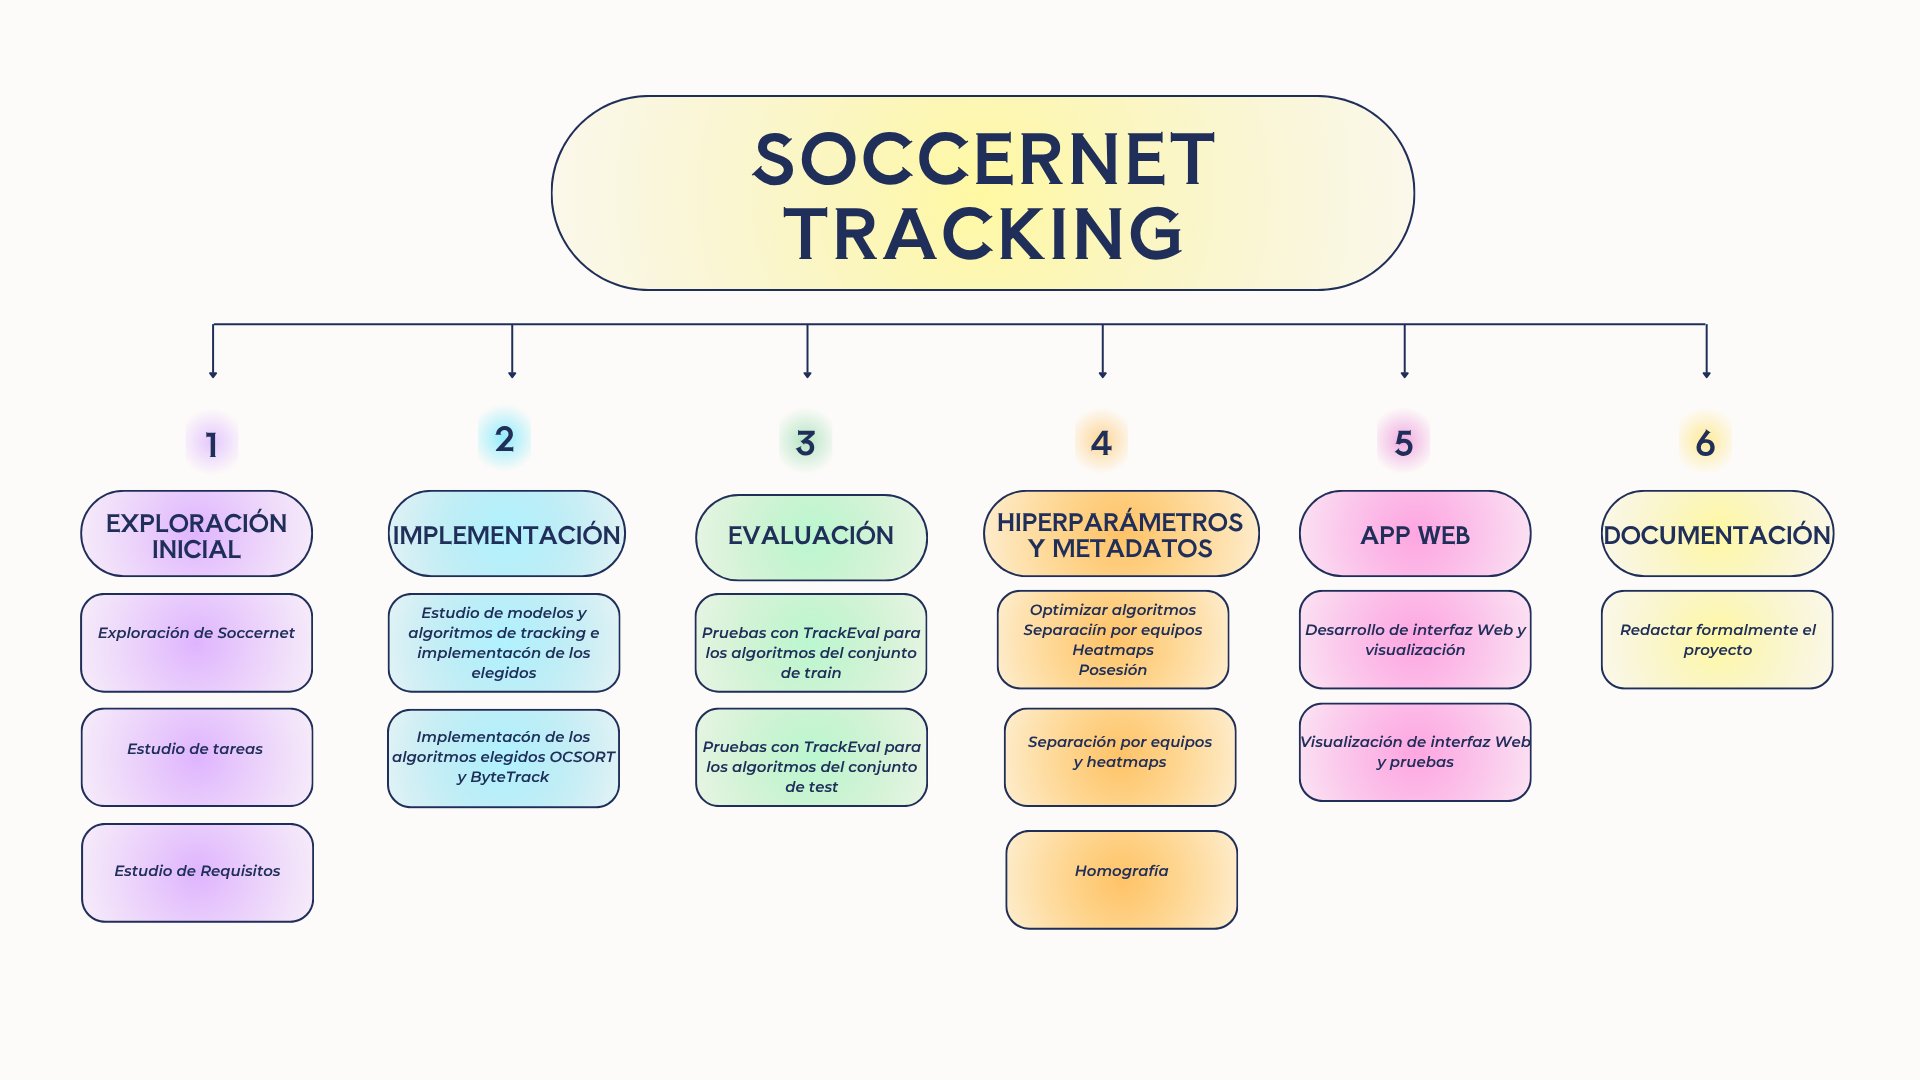
\includegraphics[width=0.98\textwidth]{figures/edt.png}
\caption{Estructura de descomposición del trabajo (EDT) del proyecto.}
\label{fig:gestion-edt}
\end{figure}

Cada paquete de trabajo del nivel inferior se detalla en el llamado
diccionario de la EDT, que recoge para cada uno su descripción, el rol
responsable y las horas dedicadas. La
Tabla~\ref{tab:gestion-edt-diccionario} recoge este diccionario completo,
ya consolidado con las horas realmente dedicadas al cierre del proyecto,
no solo las previstas en la planificación inicial, ampliadas en varios
paquetes por las causas descritas en la
sección~\ref{subsec:gestion-revision}; las horas por rol coinciden,
sumadas, con las horas totales por rol de la
Tabla~\ref{tab:gestion-costes-personal} de la
sección~\ref{sec:gestion-presupuesto}.

\begin{table}[htp]
\centering
\caption{Diccionario de la EDT: paquetes de trabajo, rol responsable y horas totales.}
\label{tab:gestion-edt-diccionario}
\small
\renewcommand{\arraystretch}{1.1}
\begin{tabular}{|p{1.0cm}|p{4.6cm}|p{3.6cm}|p{1.4cm}|}
\hline
\rowcolor{gray!25}
\textbf{ID} & \textbf{Paquete de trabajo} & \textbf{Rol} & \textbf{Horas} \\
\hline
0.1 & Traslados y reconfiguración del entorno de desarrollo (portátil,
  sobremesa, macOS) & Desarrollador & 10\,h \\
\hline
1.1 & Exploración de tareas de SoccerNet, valoración de alternativas y
  primeras pruebas de visualización & Ingeniero de Visión Artificial & 20\,h \\
\hline
1.2 & Comprensión del formato del dataset
  & Ingeniero de Visión Artificial & 5\,h \\
\hline
1.3 & Análisis de requisitos &
  Analista de software & 15\,h \\
\hline
2.1 & Implementación de ByteTrack y OC-SORT sobre \texttt{boxmot} &
  Ingeniero de Visión Artificial & 15\,h \\
\hline
2.2 & Filtrado geométrico del balón y ejecución batch sobre train &
  Ingeniero de Visión Artificial & 10\,h \\
\hline
3.1 & Integración de TrackEval y evaluación sobre train &
  Ingeniero de Visión Artificial & 20\,h \\
\hline
3.2 & Evaluación sobre test &
  Ingeniero de Visión Artificial & 10\,h \\
\hline
4.1 & Estudio de hiperparámetros de ByteTrack &
  Ingeniero de Visión Artificial & 10\,h \\
\hline
4.2 & Estudio de hiperparámetros de OC-SORT &
  Ingeniero de Visión Artificial & 10\,h \\
\hline
5.1 & Clasificación de equipos y mapas de calor (con y sin homografía) &
  Ingeniero de Visión Artificial & 20\,h \\
\hline
5.2 & Homografía real (distancia/velocidad) y posesión de balón &
  Ingeniero de Visión Artificial & 23\,h \\
\hline
6.1 & Desarrollo de la aplicación web & Desarrollador & 20\,h \\
\hline
6.2 & Ajustes y revisión de la aplicación web &
  Desarrollador & 15\,h \\
\hline
7.1 & Organización del repositorio y corrección de errores &
  Desarrollador & 20\,h \\
\hline
8.1 & Redacción de la memoria & Jefe de proyecto & 90\,h \\
\hline
\rowcolor{gray!10}
 & \textbf{Total} & & \textbf{313\,h} \\
\hline
\end{tabular}
\end{table}

Esta cifra final, superior a las 300\,h estimadas en la planificación
inicial (sección~\ref{sec:gestion-planificacion}), no es un error de
previsión menor sino el reflejo de cómo evolucionó realmente el proyecto:
la sección~\ref{subsec:gestion-revision} detalla las causas concretas de
esa desviación de horas.

\section{Planificación temporal}
\label{sec:gestion-planificacion}

\subsection{Elaboración del plan de trabajo}

El proyecto arrancó a finales de febrero de 2026 con una toma de contacto
muy preliminar con la web de SoccerNet, seguida en marzo de una fase ya
informal pero más concreta de exploración de las distintas tareas de su
ecosistema (sección~\ref{sec:gestion-fases}), antes de comprometerse
formalmente con el tracking como tarea del proyecto a finales de abril. A
partir de ahí,
la disponibilidad de tiempo fue muy variable a lo largo de los meses
siguientes debido al solapamiento con la época de exámenes del resto de
asignaturas del grado. Esta irregularidad, previsible desde el principio
dado el calendario académico, condicionó la forma de planificar: en lugar
de repartir el esfuerzo de manera uniforme mes a mes, la planificación
inicial --elaborada ya en abril, una vez elegida la tarea-- asumió
explícitamente periodos de baja dedicación durante los exámenes de mayo y
concentró el grueso del trabajo en los meses sin solapamiento académico.
Esa planificación inicial fue la siguiente:

\begin{itemize}
  \item \textbf{Abril (20--30)} -- Arranque. Exploración de tareas y
        elección definitiva de la tarea (tracking). Primeros scripts de
        visualización. Implementación de ByteTrack y OC-SORT. Ejecución
        sobre las secuencias de entrenamiento. Preparación del entorno de
        evaluación con TrackEval.
  \item \textbf{Mayo} -- Ritmo muy reducido por exámenes (aproximadamente
        20 horas en todo el mes, con prácticamente inactividad entre el 7 y
        el 25). Objetivo: obtener las primeras métricas reales y mantener
        un feedback constante de seguimiento con el tutor.
  \item \textbf{Junio} -- Núcleo del proyecto (unas 120 horas estimadas):
        evaluación en test, estudio de hiperparámetros, pipeline de
        metadatos, y comienzo de la redacción de la memoria en paralelo.
  \item \textbf{Julio} -- Cierre (unas 80 horas estimadas): desarrollo de la
        aplicación web y finalización de la memoria.
\end{itemize}

La estimación total de esta planificación inicial fue de unas 300 horas,
que incluían un margen reservado para imprevistos y tiempo de tutorías,
con una fecha de entrega prevista a finales de julio
de 2026. La Tabla~\ref{tab:gestion-gantt} representa esta misma
planificación en forma de cronograma, situando cada fase del proyecto
(sección~\ref{sec:gestion-fases}) sobre el mes o los meses en que se ha
concentrado su desarrollo, incluyendo la revisión de la planificación
descrita en la sección~\ref{subsec:gestion-revision}.

\begin{table}[htp]
\centering
\caption[Cronograma real del proyecto por fase y mes]{Cronograma real
del proyecto por fase y mes. El tono claro distingue actividad parcial o
de repaso/retoque frente al grueso del trabajo de cada fase (tono
oscuro).}
\label{tab:gestion-gantt}
\renewcommand{\arraystretch}{1.3}
\begin{tabular}{|p{3.2cm}|c|c|c|c|c|c|c|c|c|}
\hline
\rowcolor{gray!25}
\textbf{Fase} & \textbf{Feb} & \textbf{Mar} & \textbf{Abr} & \textbf{May} & \textbf{Jun} & \textbf{Jul} & \textbf{Ago} & \textbf{Sep} & \textbf{Oct} \\
\hline
1. Exploración inicial & \cellcolor{blue!10}\checkmark & \cellcolor{blue!25}\checkmark & & & & & & & \\
\hline
2. Implementación de trackers & & & \cellcolor{blue!25}\checkmark & & & & & & \\
\hline
3. Evaluación & & & \cellcolor{blue!25}\checkmark & \cellcolor{blue!25}\checkmark & & & & & \\
\hline
4. Estudio de hiperparámetros & & & & & \cellcolor{blue!25}\checkmark & & & & \\
\hline
5. Pipeline de metadatos & & & & & \cellcolor{blue!25}\checkmark & & & & \\
\hline
6. Aplicación web & & & & & & & \cellcolor{blue!25}\checkmark & \cellcolor{blue!10}\checkmark & \\
\hline
7. Redacción de la memoria & & & & & \cellcolor{blue!10}\checkmark & \cellcolor{blue!10}\checkmark & \cellcolor{blue!25}\checkmark & \cellcolor{blue!25}\checkmark & \cellcolor{blue!10}\checkmark \\
\hline
\end{tabular}
\end{table}

Como refleja el cronograma, la fase 1 tampoco se concentra en un único
mes: arranca con una toma de contacto muy ligera en febrero y se
convierte en la exploración real, ya concreta, en marzo. La fase 7
sigue un patrón parecido: arranca de forma parcial en junio y julio, se
convierte en
el grueso real del trabajo en agosto y septiembre, y se cierra con una
revisión final en octubre antes de la entrega. La fase 6 sigue un patrón
similar a menor escala: el desarrollo principal de la aplicación web se
concentra en agosto, con un repaso final en septiembre --organización del
repositorio y revisión de la interfaz-- ya en paralelo a la recta final
de la redacción
(sección~\ref{subsec:impl-web-frontend} del
capítulo~\ref{cap:implementacion}).

\subsection{Seguimiento y monitorización}
\label{subsec:gestion-monitorizacion}

\FloatBarrier

El seguimiento del tiempo dedicado a este proyecto se ha apoyado en una
herramienta de \emph{time-tracking} dedicada, Clockify (Figuras~\ref{fig:gestion-monitorizacion}
a~\ref{fig:gestion-clockify-sep-p2}), complementada por el documento de
anotaciones descrito en la sección~\ref{sec:gestion-metodologia} y por el
historial de commits del repositorio Git, cuya fecha permite además
reconstruir con razonable precisión cuándo se completó cada hito. Las
horas totales por paquete de trabajo de la Tabla~\ref{tab:gestion-edt-diccionario}
y la desviación cuantificada en la sección~\ref{subsec:gestion-revision}
proceden de esta herramienta. Para cada mes se muestran, en dos capturas
sucesivas, el reparto diario de horas junto con la categoría de proyecto
a la que pertenecen (\emph{Implementación}, \emph{Investigación} o
\emph{Redacción}), y el desglose completo de las tareas individuales
registradas con su tiempo dedicado.

\begin{figure}[htp]
\centering
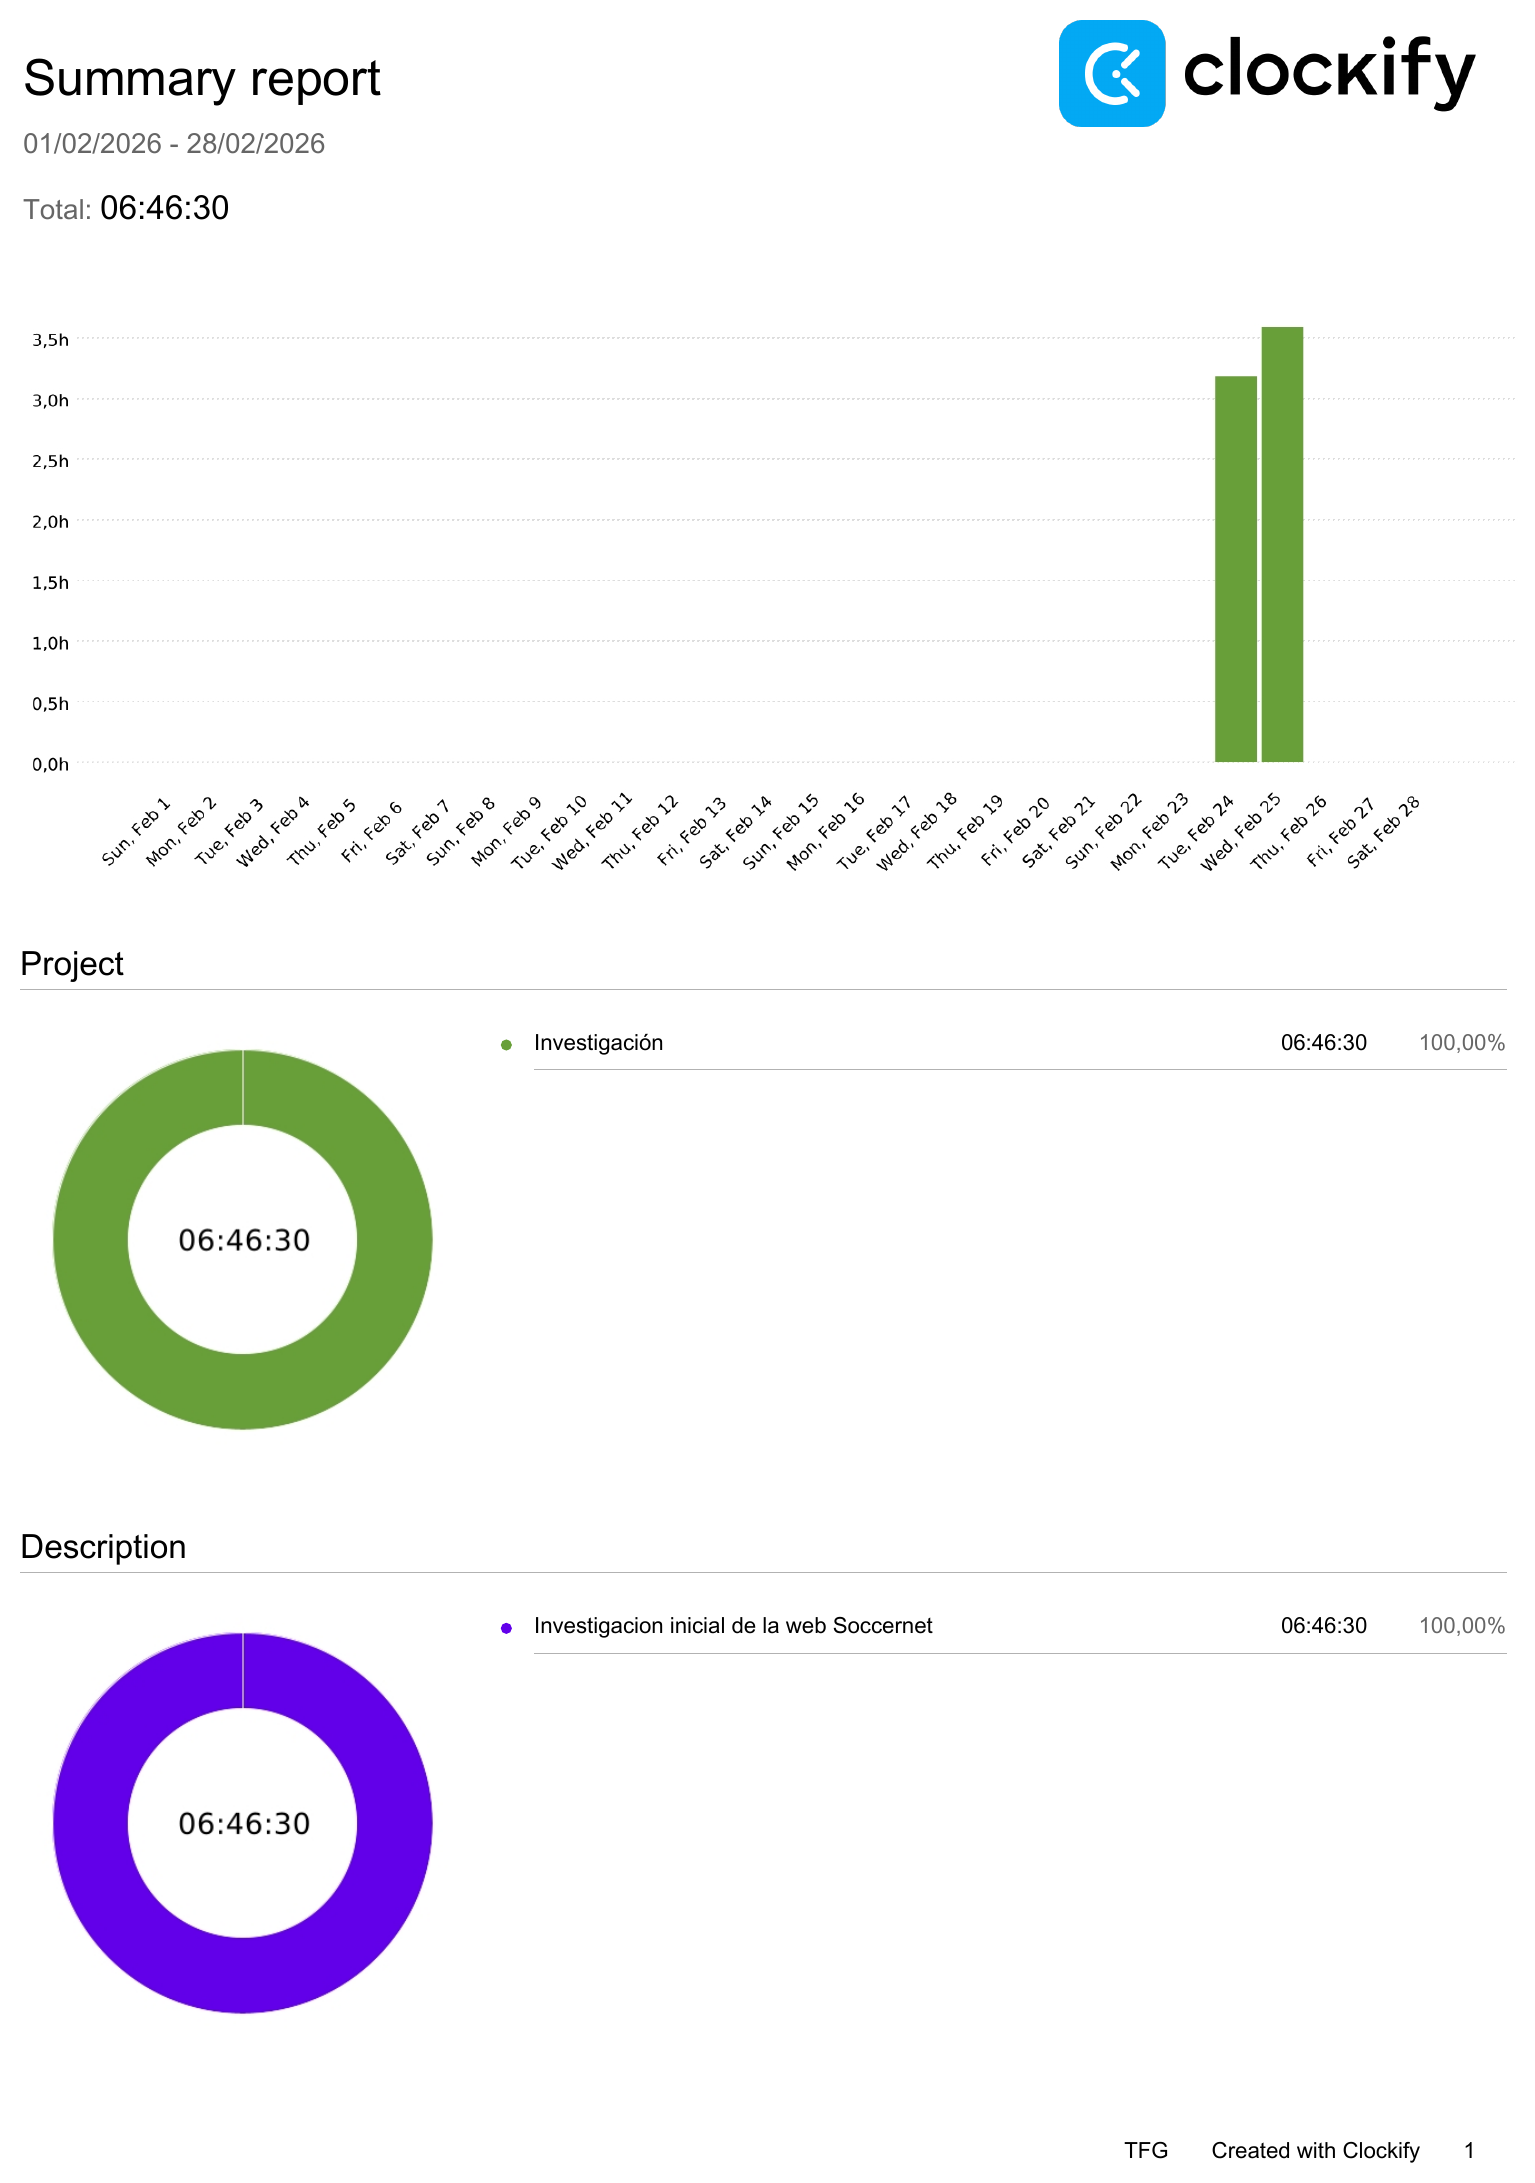
\includegraphics[height=0.72\textheight, keepaspectratio]{figures/clockify_02_2026_p1.png}
\caption{Febrero 2026: apenas 7\,h registradas, una toma de contacto muy
preliminar con la web de SoccerNet, antes de arrancar con la exploración
ya concreta de marzo.}
\label{fig:gestion-monitorizacion}
\end{figure}

\FloatBarrier

\begin{figure}[htp]
\centering
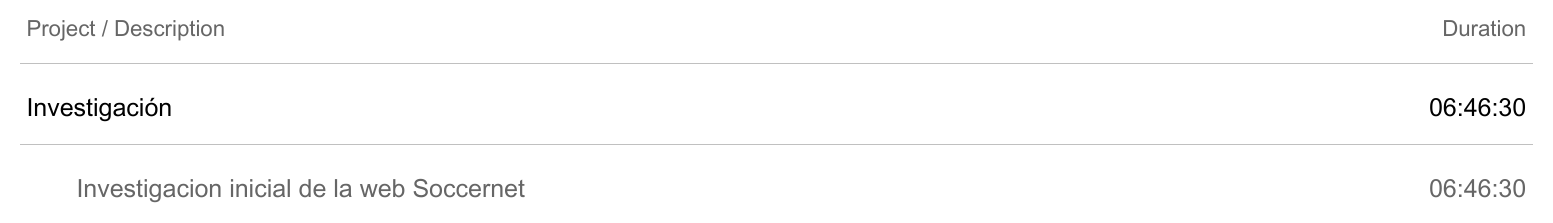
\includegraphics[width=0.92\textwidth, keepaspectratio]{figures/clockify_02_2026_p2.png}
\caption{Febrero 2026: única tarea registrada en todo el mes.}
\end{figure}

\FloatBarrier

\begin{figure}[htp]
\centering
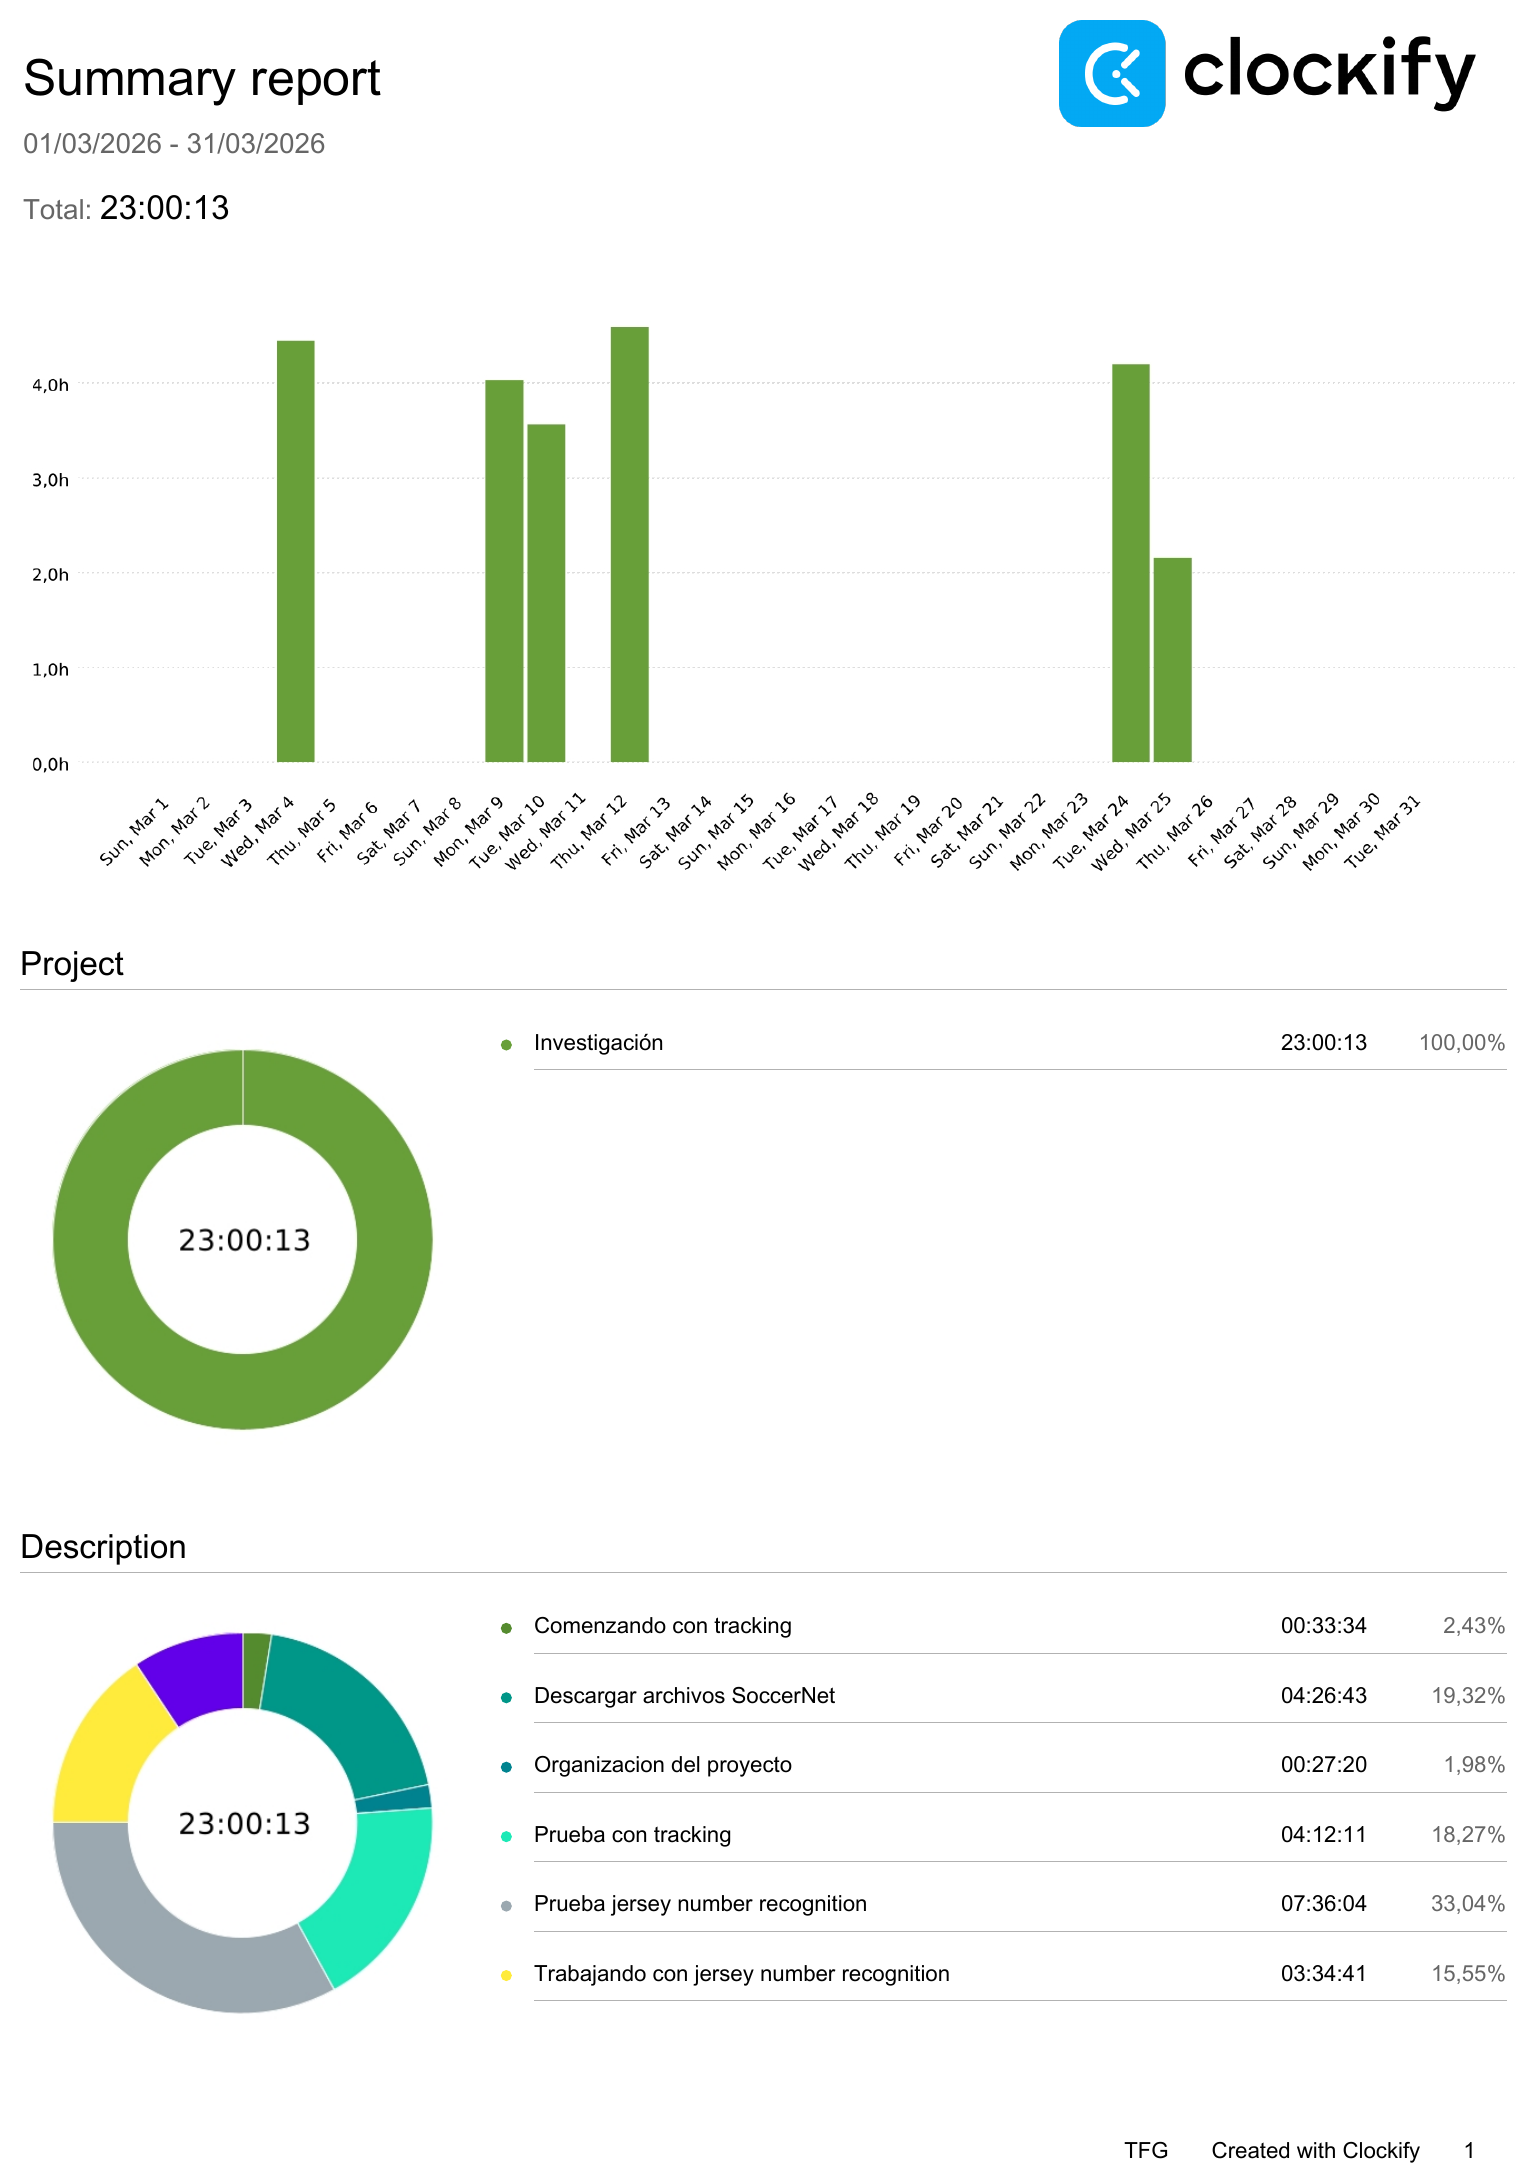
\includegraphics[height=0.72\textheight, keepaspectratio]{figures/clockify_03_2026_p1.png}
\caption{Marzo 2026: unas 23\,h registradas.}
\end{figure}

\FloatBarrier

\begin{figure}[htp]
\centering
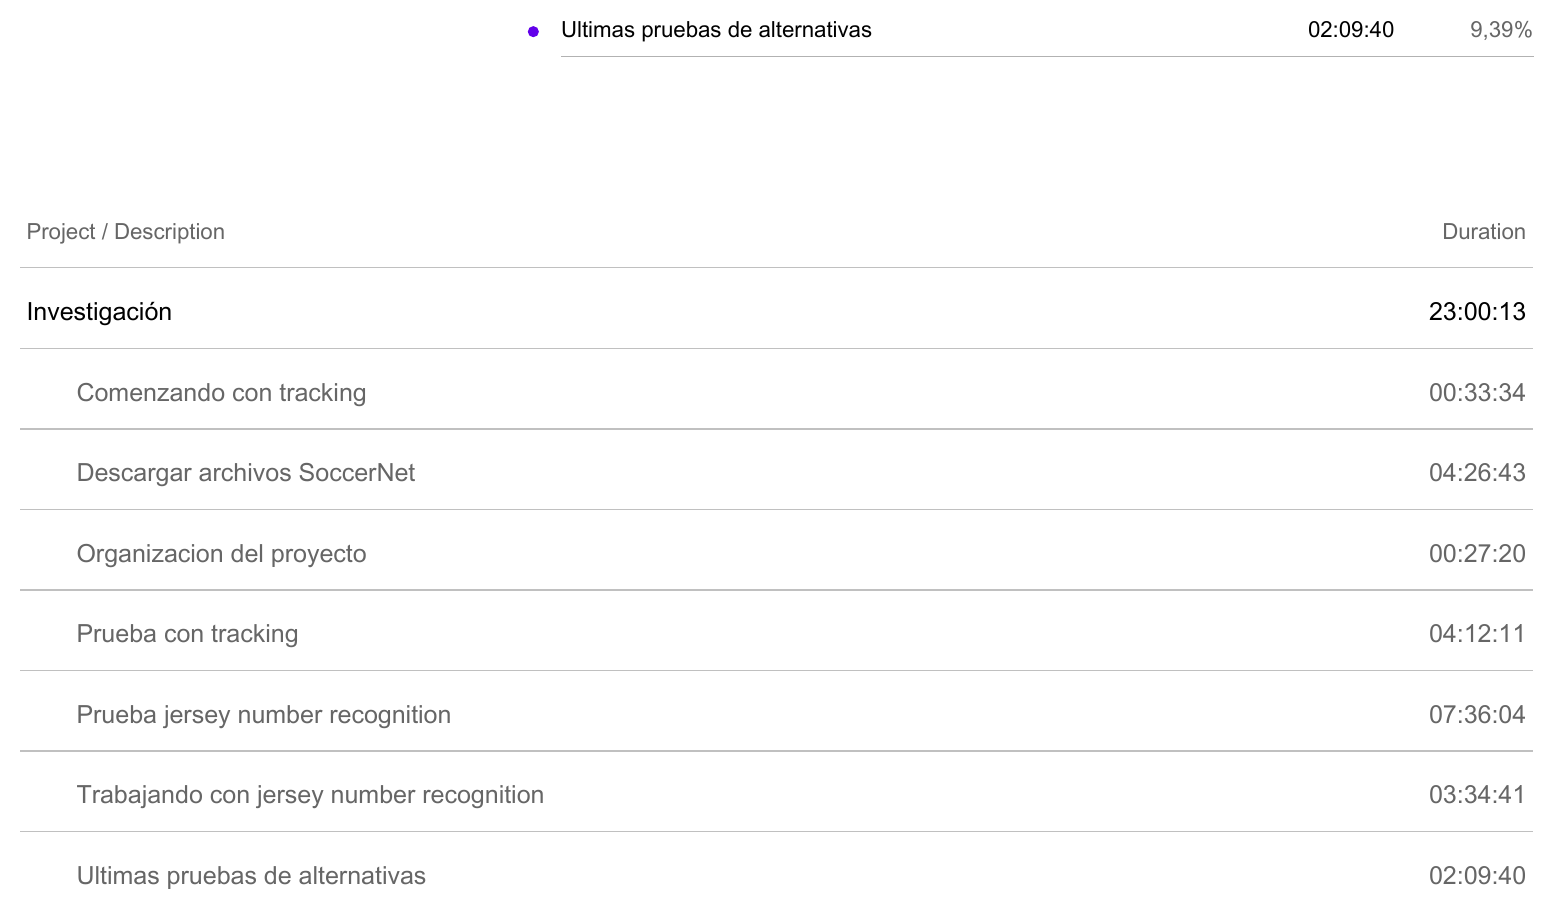
\includegraphics[width=0.92\textwidth, keepaspectratio]{figures/clockify_03_2026_p2.png}
\caption{Marzo 2026: desglose completo de las tareas de exploración
inicial y el tiempo dedicado a cada una.}
\end{figure}

\FloatBarrier

\begin{figure}[htp]
\centering
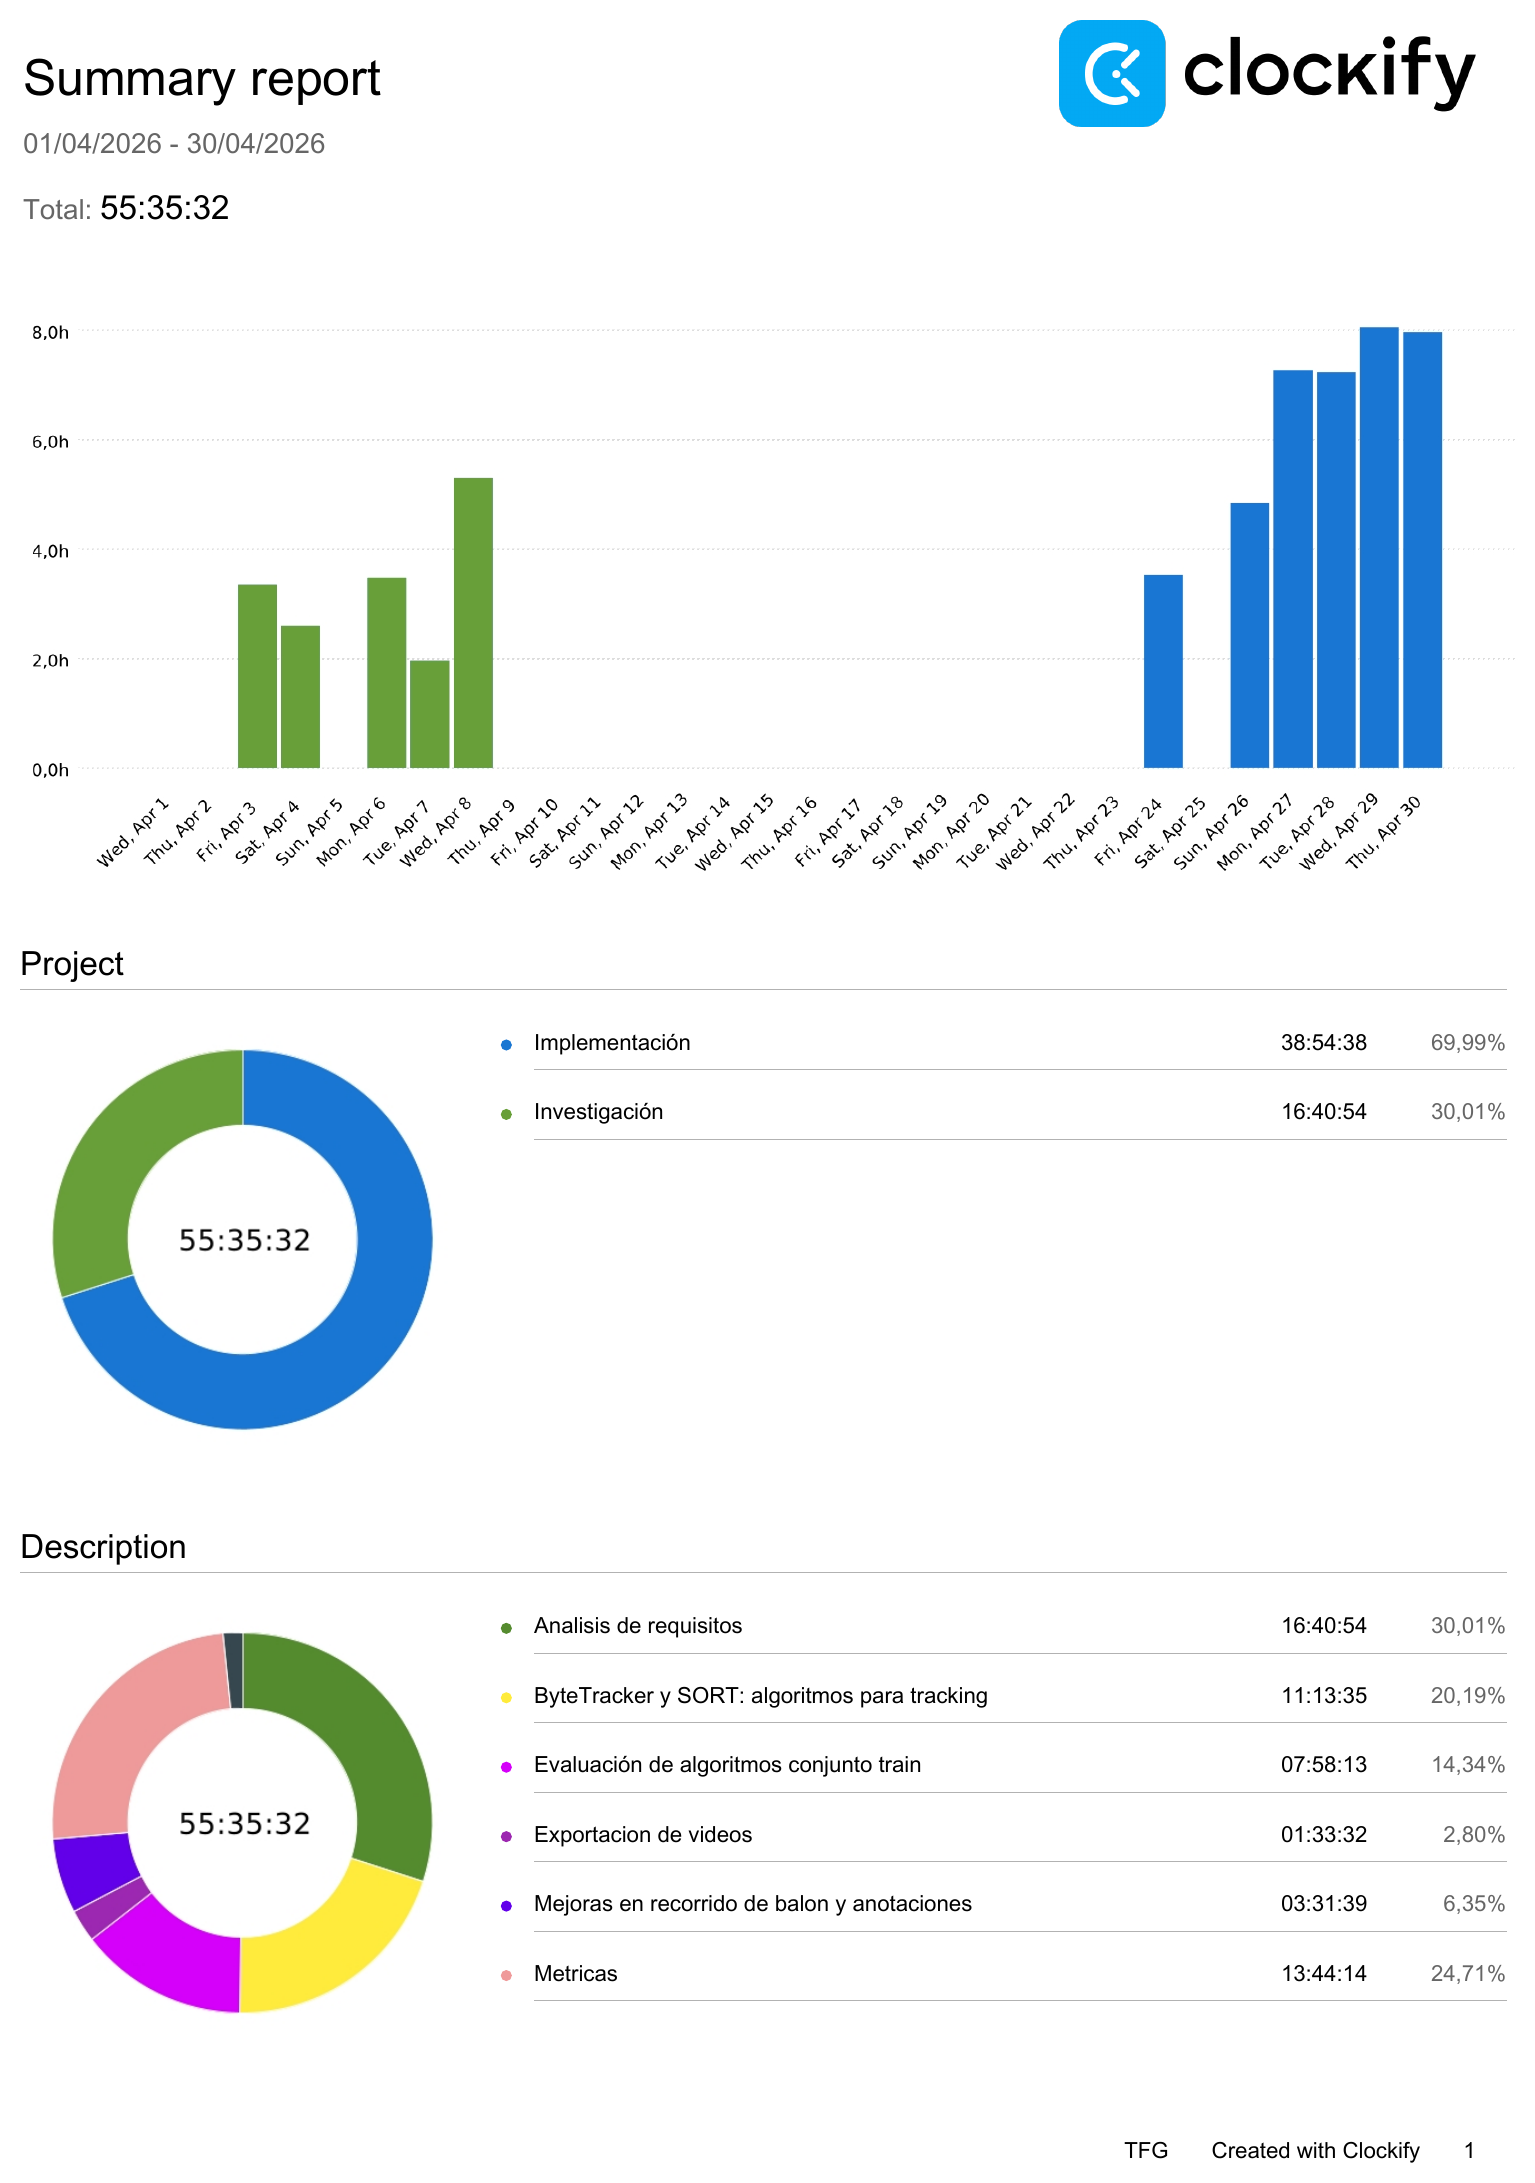
\includegraphics[height=0.72\textheight, keepaspectratio]{figures/clockify_04_2026_p1.png}
\caption{Abril 2026: unas 56\,h registradas.}
\end{figure}

\FloatBarrier

\begin{figure}[htp]
\centering
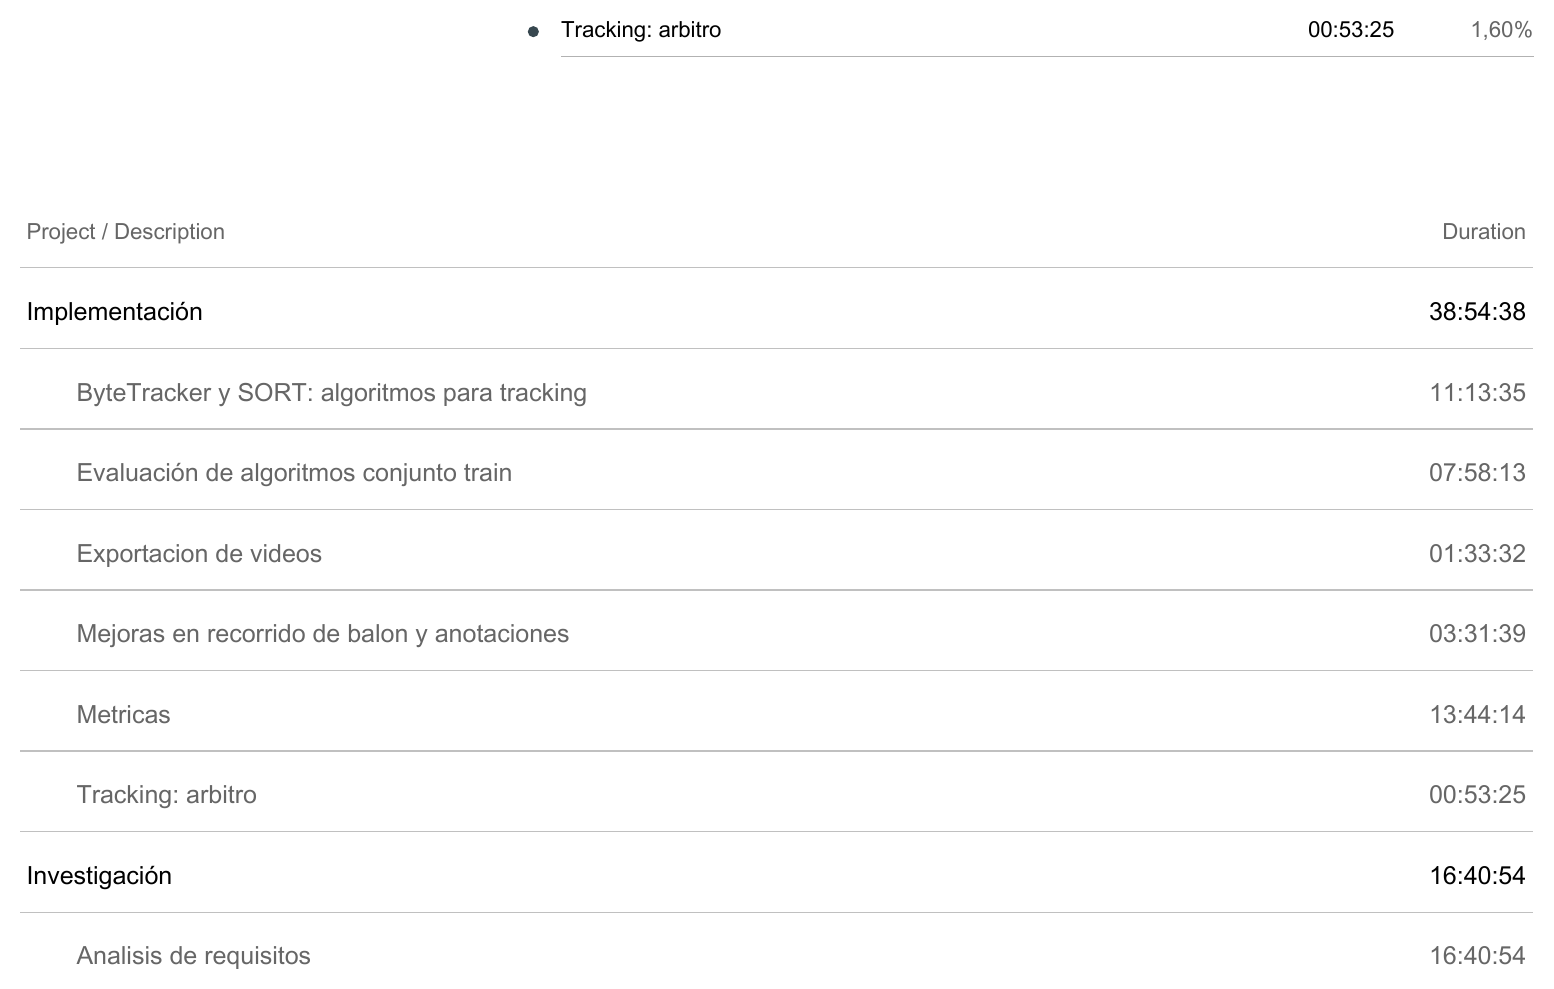
\includegraphics[width=0.92\textwidth, keepaspectratio]{figures/clockify_04_2026_p2.png}
\caption{Abril 2026: desglose completo de tareas.}
\end{figure}

\FloatBarrier

\begin{figure}[htp]
\centering
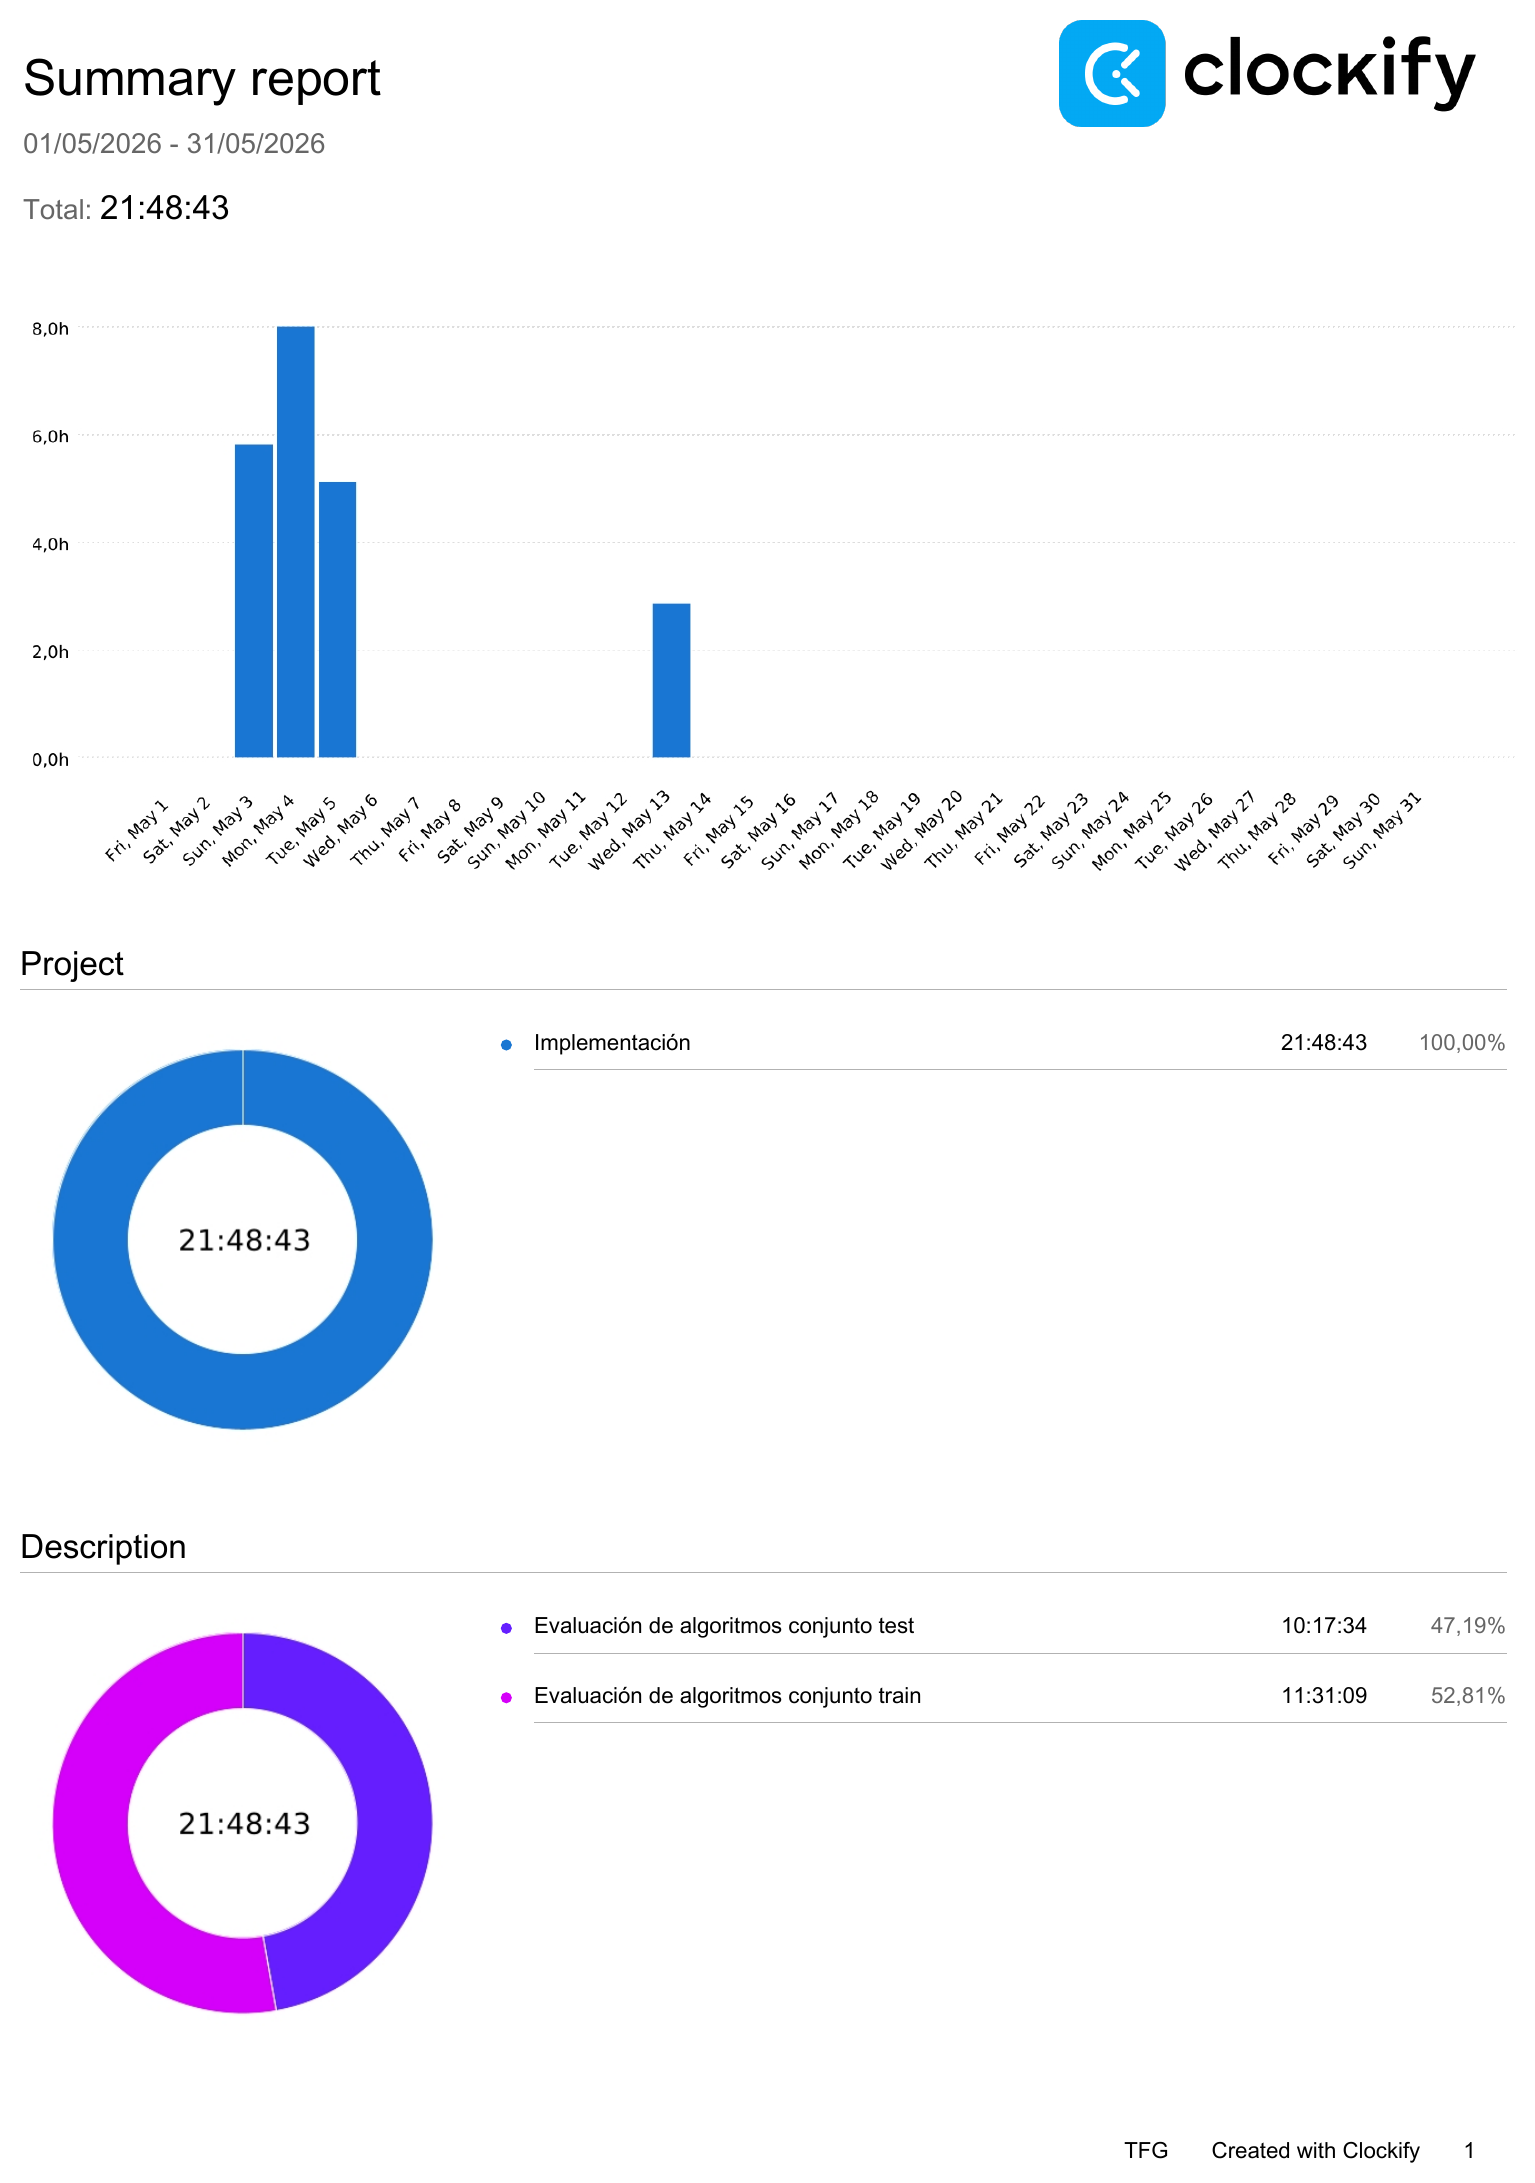
\includegraphics[height=0.72\textheight, keepaspectratio]{figures/clockify_05_2026_p1.png}
\caption{Mayo 2026: unas 22\,h registradas.}
\end{figure}

\FloatBarrier

\begin{figure}[htp]
\centering
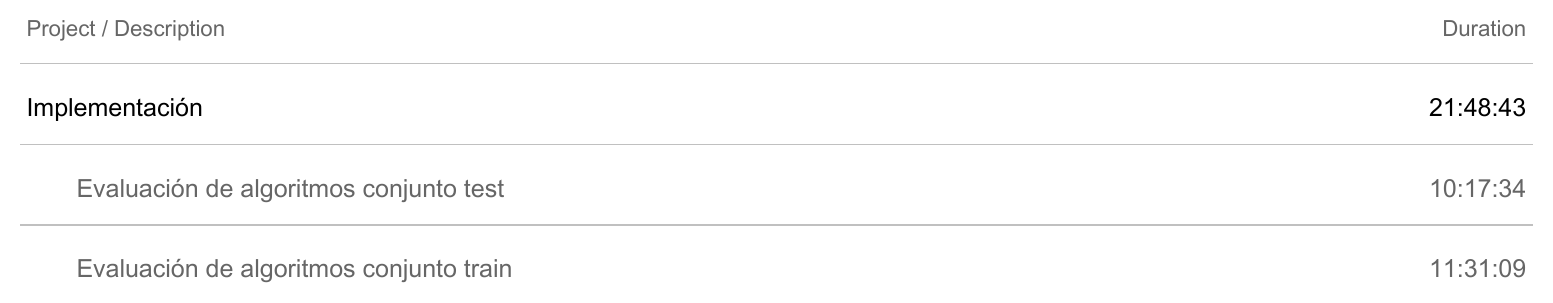
\includegraphics[width=0.92\textwidth, keepaspectratio]{figures/clockify_05_2026_p2.png}
\caption{Mayo 2026: desglose completo de las dos tareas de evaluación
realizadas.}
\end{figure}

\FloatBarrier

\begin{figure}[htp]
\centering
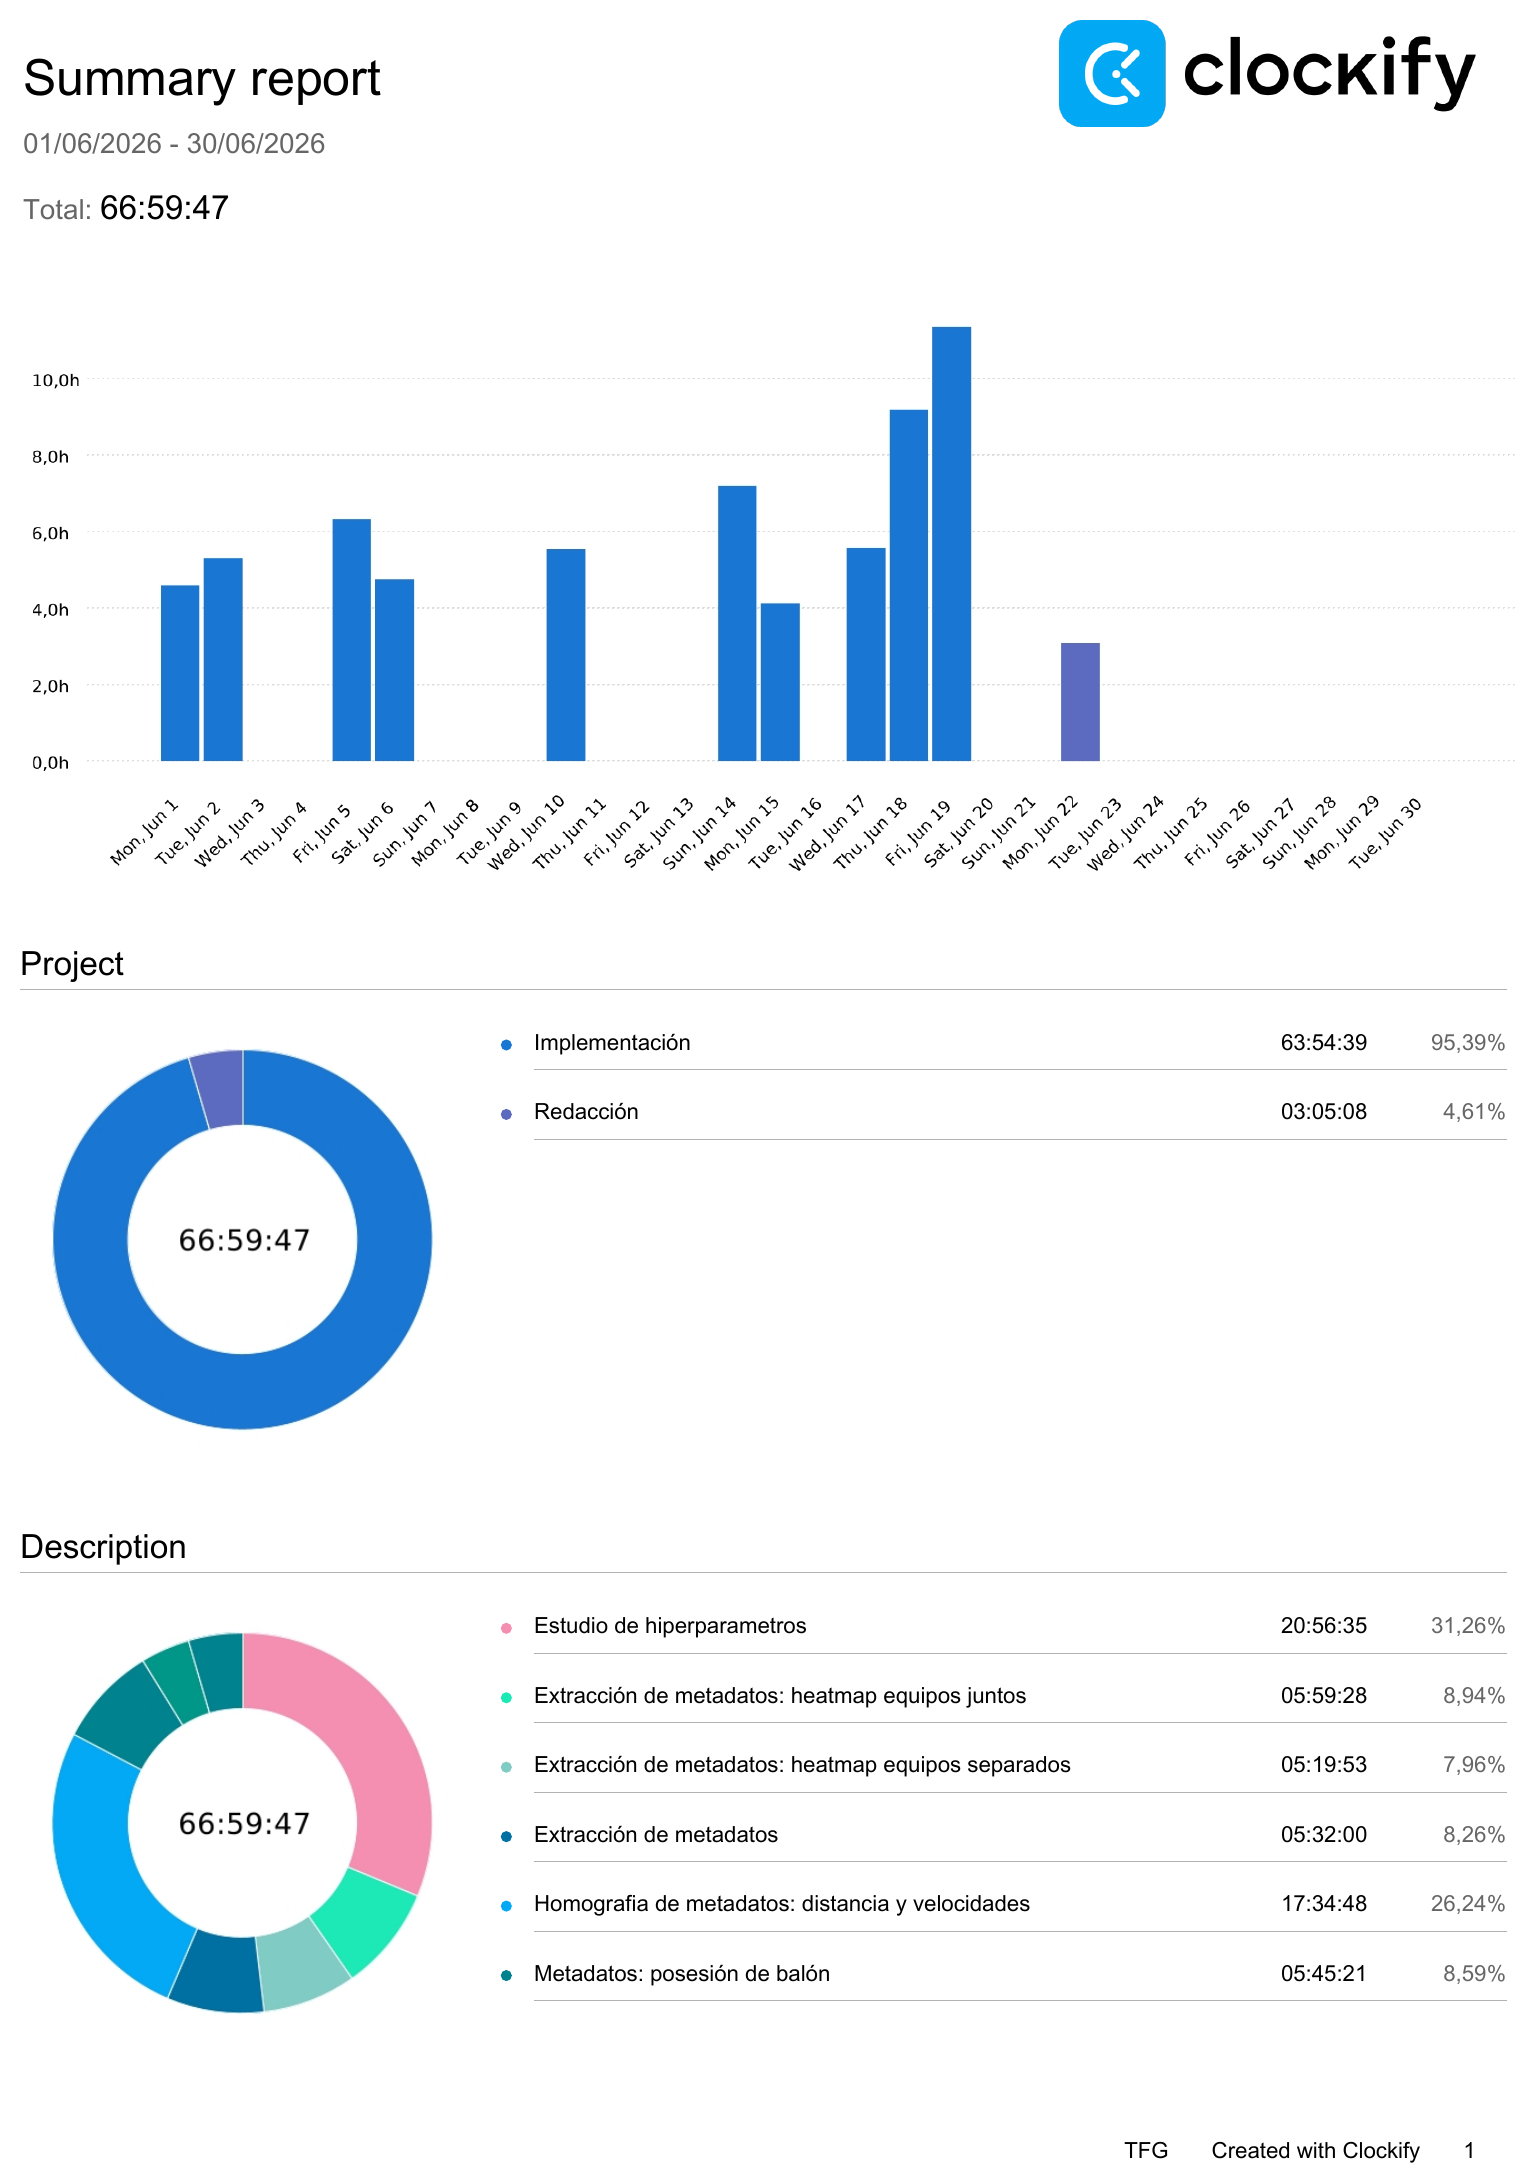
\includegraphics[height=0.72\textheight, keepaspectratio]{figures/clockify_06_2026_p1.png}
\caption{Junio 2026: cerca de 67\,h registradas.}
\end{figure}

\FloatBarrier

\begin{figure}[htp]
\centering
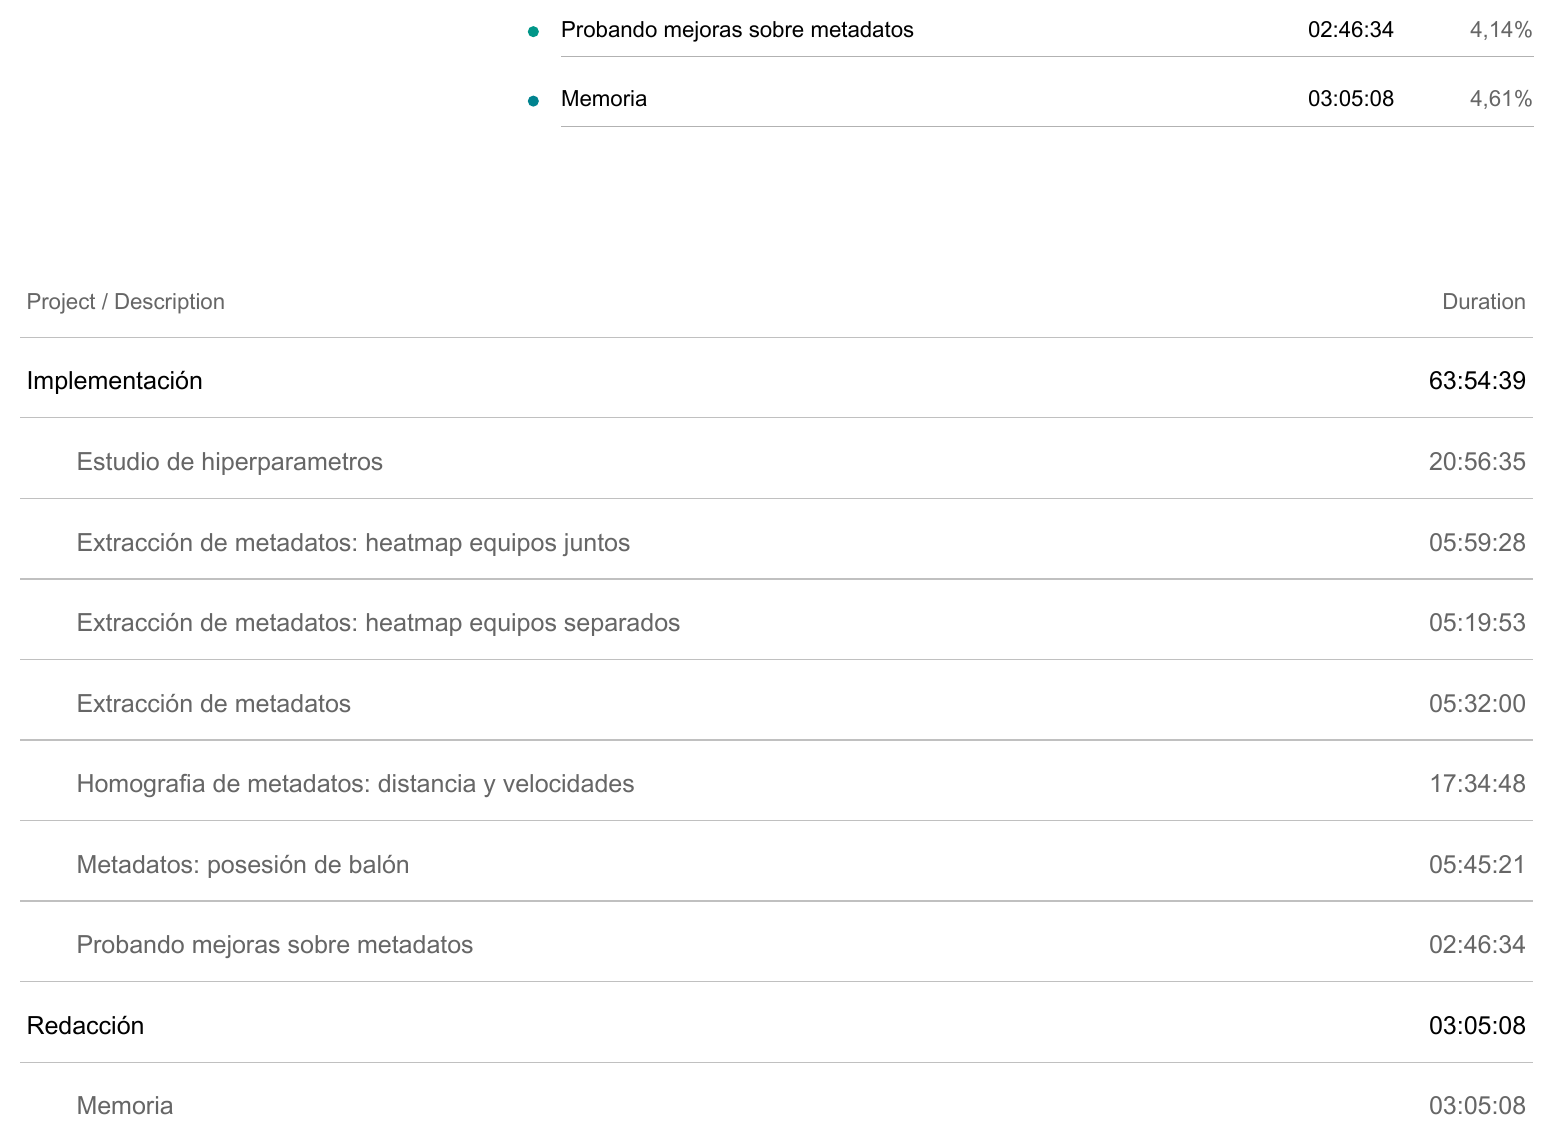
\includegraphics[width=0.92\textwidth, keepaspectratio]{figures/clockify_06_2026_p2.png}
\caption{Junio 2026: desglose completo de tareas.}
\end{figure}

\FloatBarrier

\begin{figure}[htp]
\centering
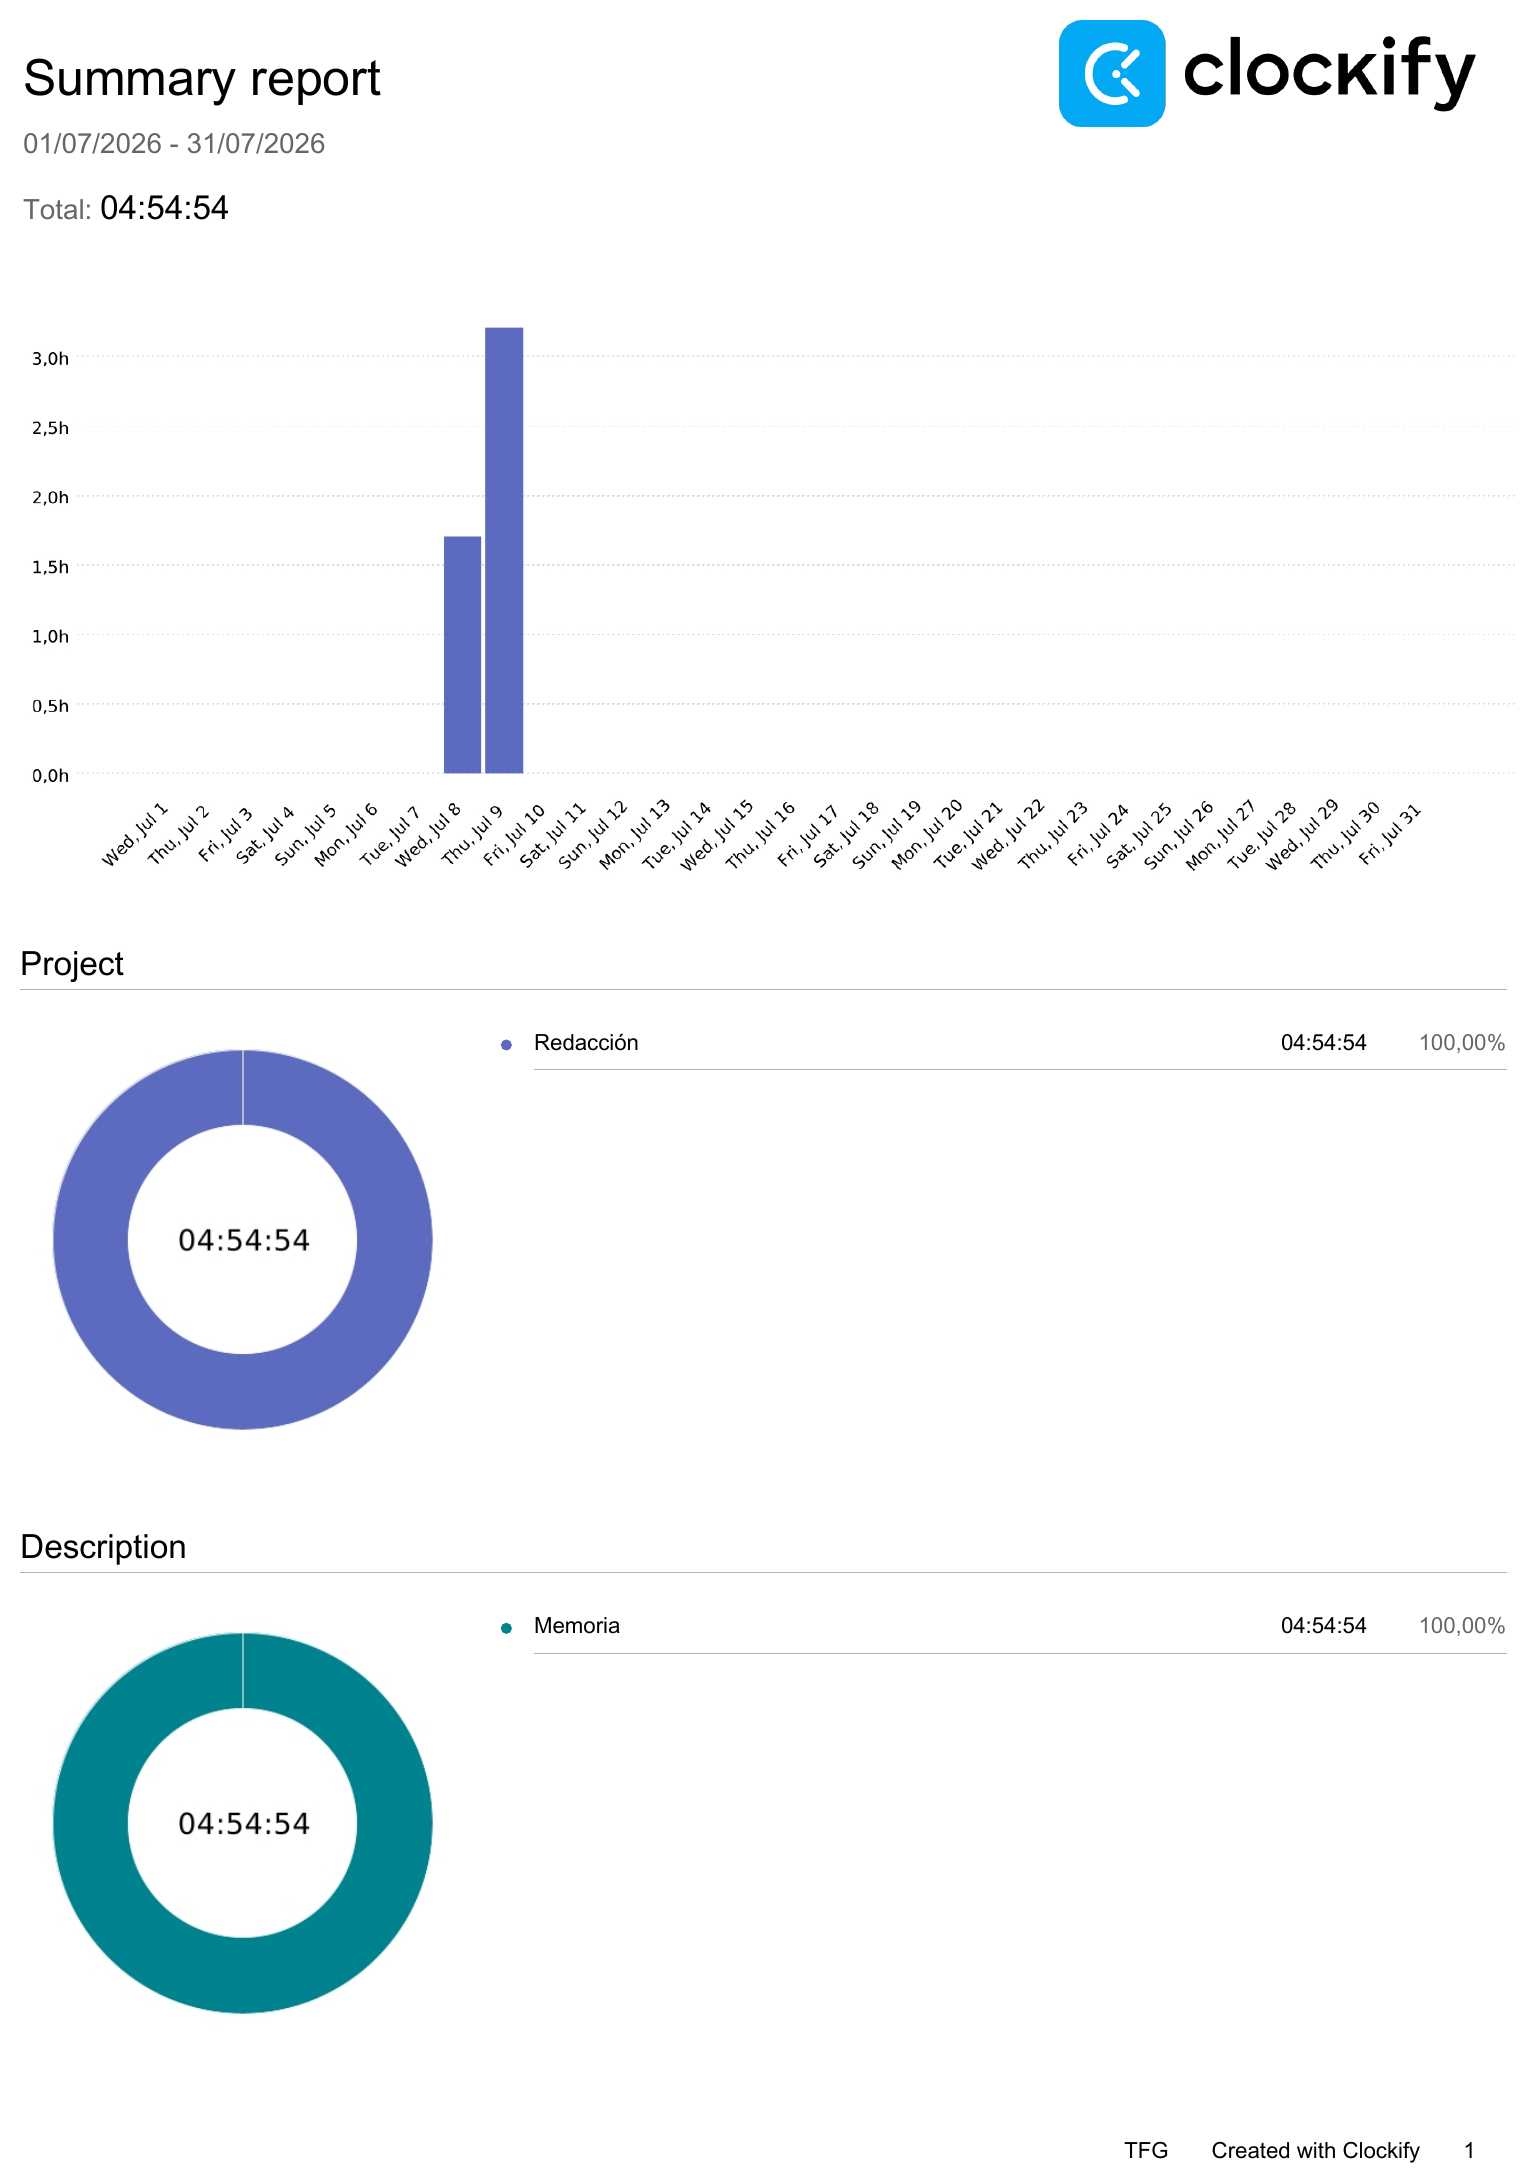
\includegraphics[height=0.72\textheight, keepaspectratio]{figures/clockify_07_2026_p1.png}
\caption{Julio 2026: apenas 5\,h registradas.}
\end{figure}

\FloatBarrier

\begin{figure}[htp]
\centering
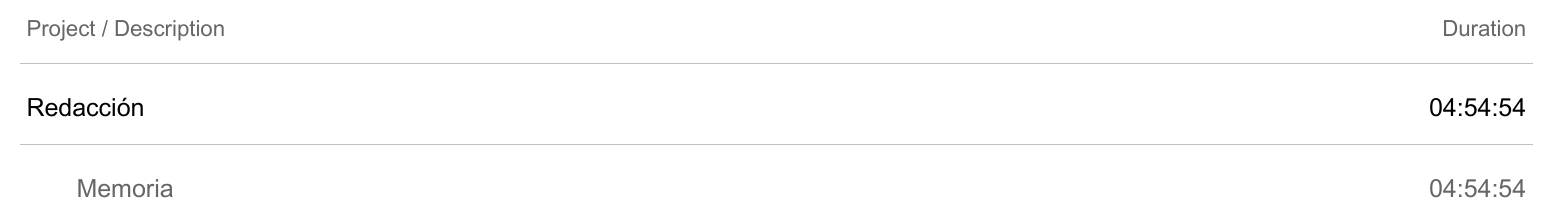
\includegraphics[width=0.92\textwidth, keepaspectratio]{figures/clockify_07_2026_p2.png}
\caption{Julio 2026: única tarea registrada en todo el mes.}
\end{figure}

\FloatBarrier

\begin{figure}[htp]
\centering
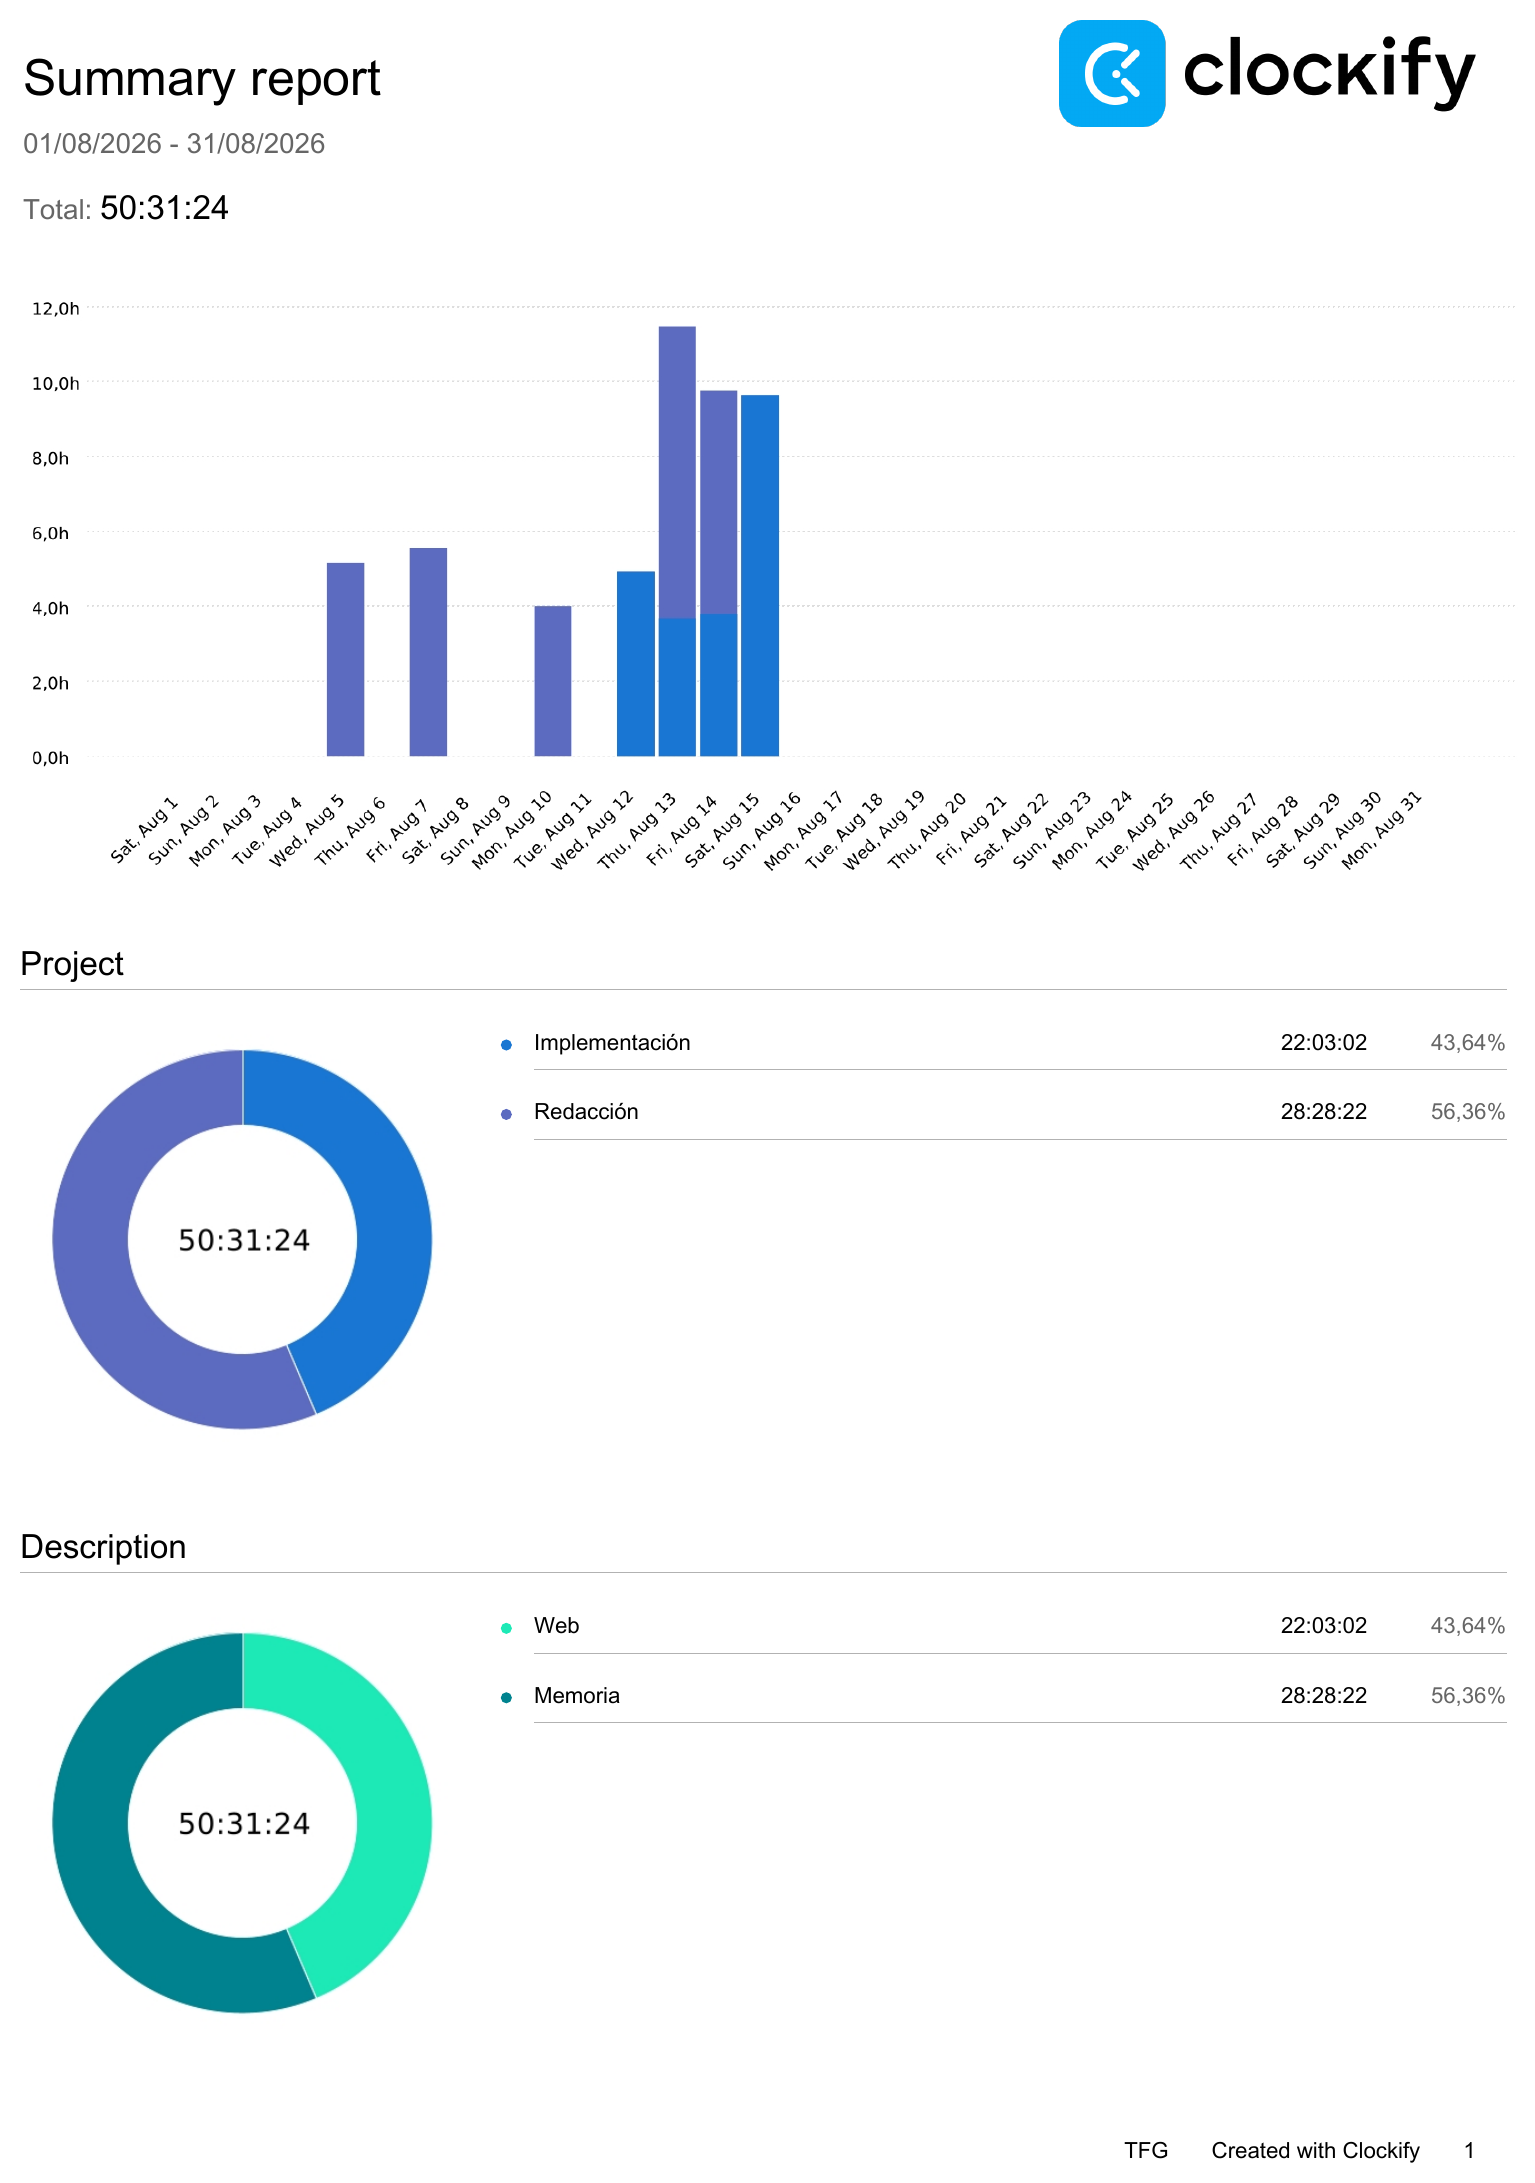
\includegraphics[height=0.72\textheight, keepaspectratio]{figures/clockify_08_2026_p1.png}
\caption{Agosto 2026: unas 51\,h registradas.}
\end{figure}

\FloatBarrier

\begin{figure}[htp]
\centering
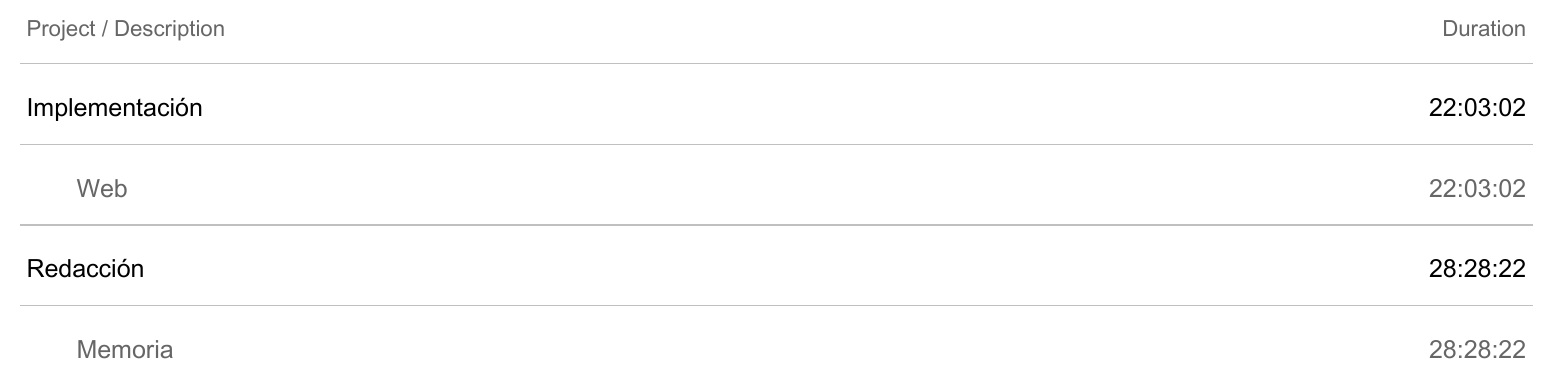
\includegraphics[width=0.92\textwidth, keepaspectratio]{figures/clockify_08_2026_p2.png}
\caption{Agosto 2026: desglose completo de tareas.}
\end{figure}

\FloatBarrier

\begin{figure}[htp]
\centering
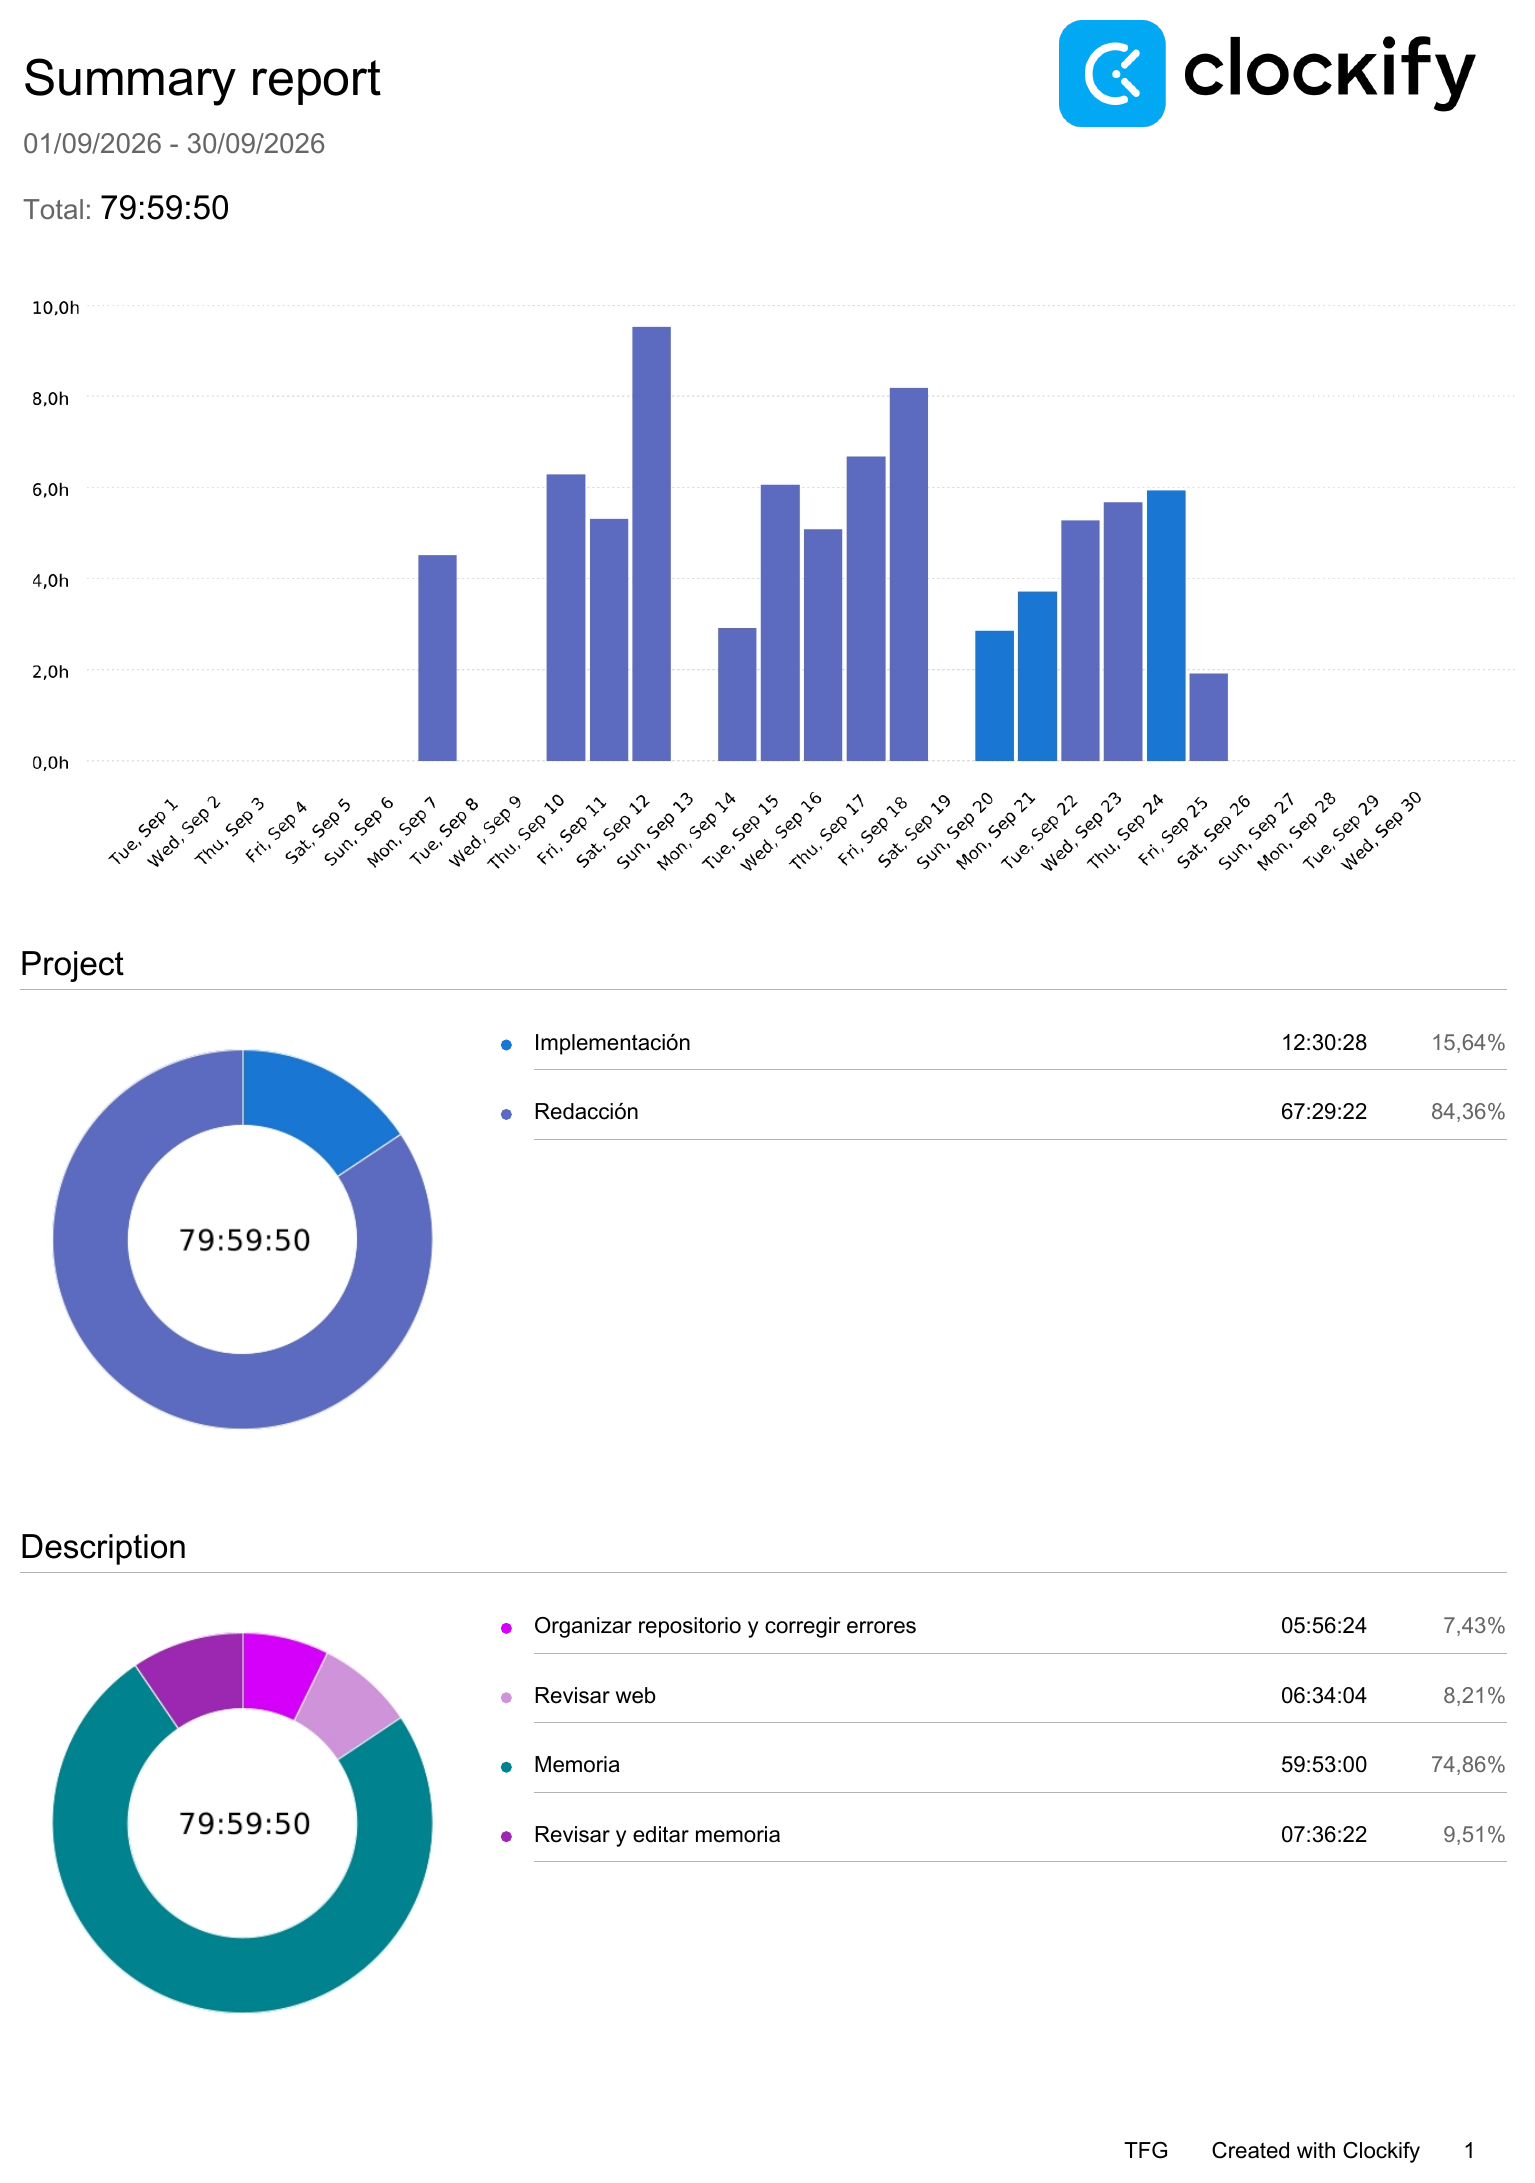
\includegraphics[height=0.72\textheight, keepaspectratio]{figures/clockify_09_2026_p1.png}
\caption{Septiembre 2026: cerca de 80\,h registradas.}
\label{fig:gestion-clockify-sep}
\end{figure}

\FloatBarrier

\begin{figure}[htp]
\centering
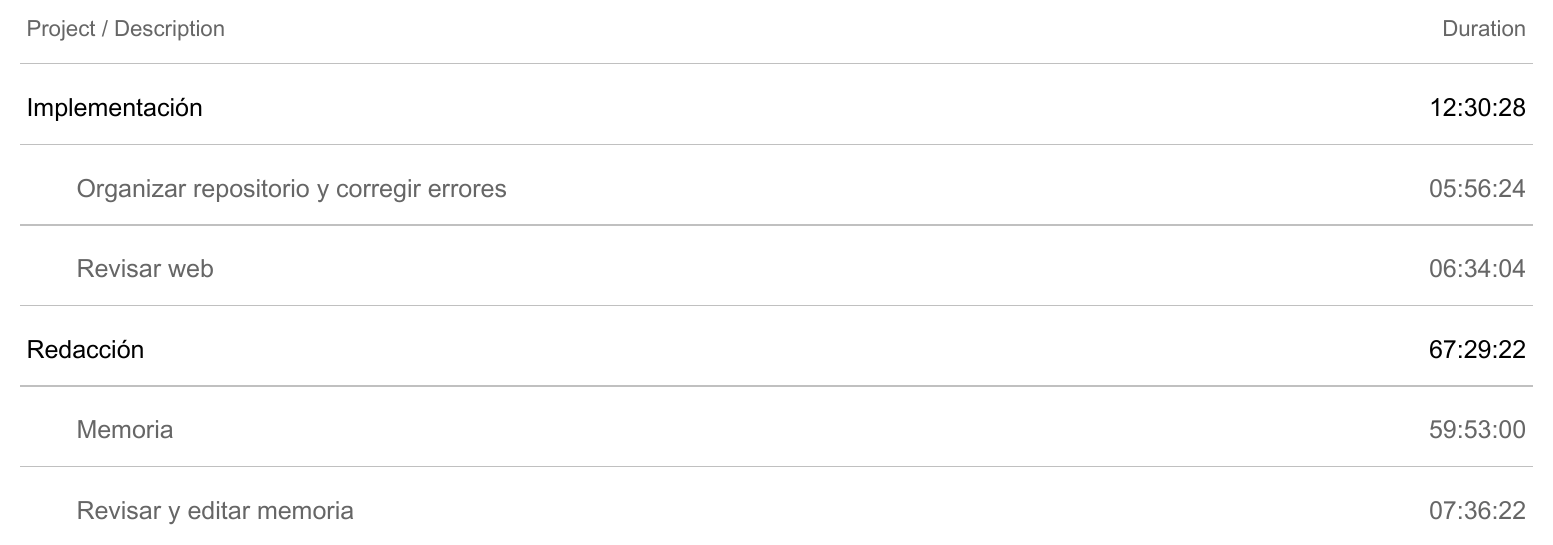
\includegraphics[width=0.92\textwidth, keepaspectratio]{figures/clockify_09_2026_p2.png}
\caption{Septiembre 2026: desglose completo de tareas.}
\label{fig:gestion-clockify-sep-p2}
\end{figure}

\FloatBarrier

\subsection{Hitos principales}

La Tabla~\ref{tab:gestion-hitos} resume los hitos principales alcanzados
hasta el cierre de este documento, reconstruidos a partir del documento de
anotaciones y del historial de commits del repositorio. Las fechas de junio
en adelante son aproximadas, ya que varias tareas se solaparon durante el
desarrollo, como es propio de la metodología iterativa descrita en la
sección~\ref{sec:gestion-metodologia}.

\begin{table}[htp]
\centering
\caption{Hitos principales del proyecto.}
\label{tab:gestion-hitos}
\renewcommand{\arraystretch}{1.3}
\begin{tabular}{|p{2.6cm}|p{9.4cm}|}
\hline
\rowcolor{gray!25}
\textbf{Fecha} & \textbf{Hito} \\
\hline
20--25 abr.\ 2026 & Exploración de tareas de SoccerNet y elección de
  tracking como tarea del proyecto. \\
\hline
26 abr.\ 2026 & OC-SORT y ByteTrack implementados sobre \texttt{boxmot}. \\
\hline
28--29 abr.\ 2026 & \texttt{run\_all\_train.py} ejecutado sobre las 57
  secuencias de train; primera evaluación con TrackEval y exportación de
  vídeos anotados. \\
\hline
Mayo 2026 & Evaluación repetida sobre el conjunto de test a petición del
  tutor; traslado del proyecto a un equipo macOS. \\
\hline
Junio 2026 & Estudio de hiperparámetros de ByteTrack y OC-SORT;
  configuración óptima encontrada para ambos algoritmos. \\
\hline
Junio 2026 & Pipeline de metadatos completo: mapa de calor general,
  clasificación de equipos por color y mapas de calor por equipo,
  homografía real sobre tramos de cámara estable (distancia y velocidad)
  y posesión de balón por proximidad. \\
\hline
Agosto 2026 & Revisión de la planificación, traslado de la entrega a la
  convocatoria de octubre; desarrollo de la aplicación web; grueso de la
  redacción sistemática de la memoria. \\
\hline
Septiembre 2026 & Continuación y grueso final de la redacción de la
  memoria, junto con la organización final del repositorio y una
  revisión de la aplicación web. \\
\hline
Octubre 2026 & Revisión final de la memoria y entrega. \\
\hline
\end{tabular}
\end{table}

\subsection{Revisión de la planificación}
\label{subsec:gestion-revision}

Como es habitual en un proyecto de esta naturaleza, la planificación
inicial no se ha cumplido de forma literal, y merece la pena detenerse en
por qué, ya que las causas de la desviación son en sí mismas informativas
sobre el trabajo realizado. Se identifican cinco causas principales,
ninguna de ellas aislada, sino acumuladas a lo largo del proyecto:

\begin{itemize}
  \item \textbf{Alcance técnico mayor de lo previsto}: el estudio de
        hiperparámetros y el pipeline de metadatos resultaron más
        extensos de lo estimado inicialmente. Cada nuevo metadato
        (clasificación de equipos, mapas de calor, homografía, posesión)
        exigió varias iteraciones de prueba y ajuste antes de dar
        resultados fiables, un coste que la planificación inicial
        (elaborada antes de conocer las dificultades reales de calibrar
        una homografía manual o de separar correctamente al árbitro en la
        clasificación por color) no pudo anticipar.
  \item \textbf{Redacción de la memoria más tardía y más costosa de lo
        previsto}: la planificación inicial contemplaba escribir la
        memoria en paralelo desde junio y cerrarla en julio
        (sección~\ref{sec:gestion-planificacion}). En la práctica, la
        redacción sistemática no arrancó en
        serio hasta agosto, y el grueso del trabajo se concentró entre
        julio y agosto, con continuación y revisión en septiembre y una
        última revisión en octubre. La documentación continua de
        decisiones y resultados intermedios, necesaria para poder
        redactar con este nivel de detalle, ha supuesto por sí misma un
        esfuerzo no contemplado en la planificación inicial.
  \item \textbf{Periodo de exámenes y viajes durante el verano}: además
        del solapamiento ya previsto con los exámenes de mayo, varios periodos de
        viaje durante el verano redujeron la disponibilidad real de
        tiempo en semanas concretas, sin que se hubiera reservado margen
        explícito para ello en la planificación inicial.
  \item \textbf{Retraso inicial por la exploración de alternativas}: la
        fase de exploración inicial de tareas de SoccerNet
         llevó más tiempo del previsto,
        al valorarse varias alternativas antes de comprometerse con el
        tracking como tarea del proyecto
        (sección~\ref{sec:analisis-decision}).
  \item \textbf{Incidencias con el equipo de desarrollo}: un problema con
        el portátil personal con el que se inició el proyecto obligó a
        migrar a un portátil macOS a mitad del desarrollo, en paralelo al
        uso ya habitual de un equipo de sobremesa, y la necesidad de
        recrear el entorno en cada cambio de equipo consumió tiempo no
        planificado.
\end{itemize}

Por este motivo, de acuerdo con el tutor, la entrega del proyecto se ha
trasladado de la convocatoria de julio a la \textbf{convocatoria de
octubre de 2026}, lo que ha permitido completar con mayor profundidad tanto
el pipeline de metadatos como la propia memoria, en lugar de recortar
alcance para cumplir la fecha original. Como consecuencia directa de estas
causas, la dedicación real asciende a las \textbf{313\,h} recogidas en el
diccionario de la EDT (Tabla~\ref{tab:gestion-edt-diccionario}), 13\,h por
encima de las 300\,h de la planificación inicial. La
Tabla~\ref{tab:gestion-desviaciones} resume las principales desviaciones
respecto al plan inicial.

\begin{table}[htp]
\centering
\caption{Principales desviaciones respecto a la planificación inicial.}
\label{tab:gestion-desviaciones}
\renewcommand{\arraystretch}{1.3}
\begin{tabular}{|p{2.6cm}|p{4.6cm}|p{4.8cm}|}
\hline
\rowcolor{gray!25}
\textbf{Elemento} & \textbf{Plan inicial} & \textbf{Desarrollo real} \\
\hline
Estudio de hiperparámetros & Barrido rápido, sin cuantificar horas de
  antemano & Varias iteraciones por algoritmo hasta encontrar una
  configuración óptima defendible \\
\hline
Pipeline de metadatos & Un mapa de calor general & Equipos, heatmaps por
  equipo, homografía (distancia/velocidad) y posesión \\
\hline
Redacción de la memoria & En paralelo desde junio, cerrada en julio &
  Primeros apuntes en junio, arranque real en julio, grueso del trabajo
  en agosto y septiembre, y revisión final en octubre \\
\hline
Aplicación web & Prevista en julio & Desarrollo principal en agosto de
  2026, tras completar el pipeline de metadatos, con un repaso final en
  septiembre (organización del repositorio y revisión de la interfaz) en
  paralelo a la redacción de los últimos capítulos de esta memoria \\
\hline
Horas totales dedicadas & 300\,h (planificación inicial) & 313\,h
  (Tabla~\ref{tab:gestion-edt-diccionario}) \\
\hline
Fecha de entrega & Convocatoria de julio de 2026 & Convocatoria de
  octubre de 2026 \\
\hline
\end{tabular}
\end{table}

\section{Entorno de desarrollo}
\label{sec:gestion-entorno}

El desarrollo se ha realizado en Python 3.11, dentro de un entorno virtual
(\texttt{venv\_tfg}) aislado dentro del propio repositorio del proyecto, con
las dependencias fijadas en \texttt{requirements.txt} para garantizar la
reproducibilidad de los resultados de forma correcta. Las herramientas principales empleadas
son OpenCV (lectura y anotación de frames), \texttt{boxmot} (implementaciones
de los algoritmos de tracking), \texttt{trackeval} (evaluación con métricas
MOT estándar), \texttt{scikit-learn} (clasificación de equipos por color
mediante K-means) y \texttt{matplotlib} (generación de gráficas y mapas de
calor). El desglose completo de versiones y la justificación de las
decisiones técnicas más relevantes sobre el entorno (incluyendo los
problemas encontrados durante su configuración) se detalla en la
sección~\ref{sec:implementacion-entorno} del capítulo~\ref{cap:implementacion}.

El proyecto se inició en un portátil personal HP Pavilion de 8 GB de RAM, y a
mitad del desarrollo se trasladó a un ordenador de sobremesa con GPU AMD
Radeon RX 6900 XT (16\,GB VRAM) como entorno principal. Un problema con el
portátil original obligó, más adelante, a migrar a un portátil macOS,
usado desde entonces en paralelo al equipo de sobremesa según la
disponibilidad; recrear el entorno de desarrollo en cada uno de estos
cambios de equipo (problema P15, sección~\ref{sec:implementacion-entorno})
consumió tiempo no contemplado en la planificación inicial. Dado que
los algoritmos de tracking utilizados en este proyecto (ByteTrack, OC-SORT)
son clásicos y no requieren redes neuronales de gran tamaño en tiempo de
inferencia, todo el desarrollo se ha realizado sobre CPU sin que ello
supusiera una limitación relevante; la GPU AMD, al no ser compatible con
CUDA, se planteó como posible aceleración para líneas de trabajo futuras que
incorporen re-identificación basada en redes neuronales.

\section{Estimación de recursos y presupuesto}
\label{sec:gestion-presupuesto}

Al tratarse de un proyecto académico individual, en este caaso Trabajo Fin de Grado, no ha existido un
presupuesto real asociado a su desarrollo. No obstante, y siguiendo la práctica habitual en
la documentación de proyectos de ingeniería del software, se presenta a continuación una estimación de
los recursos que hubiera requerido su realización en un contexto
profesional, apoyada en los cuatro roles descritos en la
sección~\ref{sec:gestion-roles} y en el diccionario de la EDT de la
sección~\ref{sec:gestion-edt}.

\subsection{Costes de personal}

Las tarifas por hora empleadas en la Tabla~\ref{tab:gestion-costes-personal}
proceden de la \textbf{Instrucción 2/2020, de 30 de junio, de la
Dirección General de Transformación Digital de la Junta de Andalucía,
sobre perfiles y precios de referencia de la contratación de bienes y
servicios TIC} \citep{andalucia2020precios}, que fija precios de
referencia (IVA excluido) para los perfiles profesionales TIC más
comunes según el acuerdo técnico europeo CWA 16458-1:2018. Como esta
instrucción no contempla un perfil específico de \emph{ingeniería de
visión artificial},
se ha usado como equivalente el perfil de \textbf{arquitecto de
sistemas}, el más próximo por nivel de especialización técnica; el resto
de roles de este proyecto sí tienen un perfil directamente equivalente
en la instrucción. La estimación se aplica sobre las horas totales
realmente dedicadas (313\,h, Tabla~\ref{tab:gestion-edt-diccionario}),
repartidas por rol de acuerdo con el diccionario de la EDT.

\begin{table}[htp]
\centering
\caption{Estimación de costes de personal sobre las 313\,h reales dedicadas al proyecto.}
\label{tab:gestion-costes-personal}
\renewcommand{\arraystretch}{1.3}
\begin{tabular}{|p{3.6cm}|p{3.4cm}|r|r|r|}
\hline
\rowcolor{gray!25}
\textbf{Rol} & \textbf{Perfil equivalente (Junta de Andalucía)} & \textbf{Horas} & \textbf{€/h} & \textbf{Coste} \\
\hline
Jefe de proyecto & Gestor de proyecto & 90\,h & 44{,}12\,€ & 3\,970{,}80\,€ \\
\hline
Analista de software & Analista de negocio & 15\,h & 33{,}17\,€ & 497{,}55\,€ \\
\hline
Ingeniero de Visión Artificial & Arquitecto de sistemas & 143\,h & 33{,}45\,€ & 4\,783{,}35\,€ \\
\hline
Desarrollador & Desarrollador & 65\,h & 25{,}67\,€ & 1\,668{,}55\,€ \\
\hline
\rowcolor{gray!10}
\textbf{Total} & & \textbf{313\,h} & & \textbf{10\,920{,}25\,€} \\
\hline
\end{tabular}
\end{table}

\subsection{Costes materiales y operacionales}

Además de los costes de personal, un proyecto de estas características
conllevaría los costes materiales y operacionales que recoge la
Tabla~\ref{tab:gestion-costes-operacionales}. La mayoría son recursos sin
coste directo, por tratarse de equipo ya disponible o de herramientas de
código abierto; el único coste realmente cuantificable es el consumo
eléctrico, calculado a partir de una potencia media de consumo de
150\,W, una cifra intermedia entre el portátil y el equipo de sobremesa
descritos en la sección~\ref{sec:gestion-entorno}, ya que no todas las
313\,h de dedicación se han realizado con el equipo de mayor consumo y
las 313\,h totales del proyecto (Tabla~\ref{tab:gestion-edt-diccionario}):
$150\,\mathrm{W} \times 313\,\mathrm{h} = 46{,}95\,\mathrm{kWh}$, que al precio
medio doméstico de la electricidad en España (en torno a 0{,}16\,€/kWh)
supone un coste estimado de \textbf{7{,}51\,€} a lo largo de todo el
proyecto.

\begin{table}[htp]
\centering
\caption{Costes materiales y operacionales estimados.}
\label{tab:gestion-costes-operacionales}
\renewcommand{\arraystretch}{1.3}
\begin{tabular}{|p{5.4cm}|p{6.4cm}|}
\hline
\rowcolor{gray!25}
\textbf{Concepto} & \textbf{Coste} \\
\hline
Hardware (equipo de desarrollo ya disponible, sin GPU dedicada necesaria,
  sección~\ref{sec:gestion-entorno}) & Sin coste incremental \\
\hline
Software y librerías (Python, OpenCV, \texttt{boxmot}, \texttt{trackeval},
  scikit-learn, matplotlib, Git) & 0\,€ (código abierto) \\
\hline
Dataset (SoccerNet-Tracking) & 0\,€ (acceso académico gratuito) \\
\hline
Asistentes de inteligencia artificial (Claude Code,
  capítulo~\ref{cap:uso-ia}) & No cuantificado en esta estimación \\
\hline
Consumo eléctrico ($150\,\mathrm{W} \times 313\,\mathrm{h} = 46{,}95\,\mathrm{kWh}$
  a 0{,}16\,€/kWh) & 7{,}51\,€ \\
\hline
\rowcolor{gray!10}
\textbf{Total cuantificado} & \textbf{7{,}51\,€} \\
\hline
\end{tabular}
\end{table}

Este bajo coste de infraestructura es, precisamente, uno de los factores que
hace atractivo el enfoque seguido en este proyecto (véase la justificación de
la elección de tarea en la sección~\ref{sec:analisis-decision}): al partir de
detecciones ya calculadas y de algoritmos de tracking clásicos disponibles
como librería, el proyecto es reproducible por terceros sin inversión en
infraestructura específica.

\subsection{Desviación respecto al coste planificado}

Como se describe en la sección~\ref{subsec:gestion-revision}, la dedicación
real (313\,h) ha superado en 13\,h la planificación inicial de 300\,h,
principalmente por el mayor alcance del estudio de hiperparámetros y del
pipeline de metadatos, y por el tiempo dedicado a documentar el proceso
con el nivel de detalle de esta memoria. A diferencia de lo que ocurriría
sin un registro fiable de horas, en este proyecto sí se ha dispuesto de
una herramienta de \emph{time-tracking} dedicada
(sección~\ref{subsec:gestion-monitorizacion}), lo que permite ofrecer una
cifra de coste real y no solo una desviación cualitativa: aplicando las
mismas tarifas de la Tabla~\ref{tab:gestion-costes-personal} sobre el
reparto por rol de las 300\,h de la planificación inicial (40\,h jefe de
proyecto, 20\,h analista, 165\,h ingeniero de Visión Artificial, 75\,h
desarrollador) y el mismo criterio de consumo eléctrico sobre esas 300\,h
($150\,\mathrm{W} \times 300\,\mathrm{h} = 45\,\mathrm{kWh}$, a
0{,}16\,€/kWh), se obtiene el coste total estimado que recoge la
Tabla~\ref{tab:gestion-costes-resumen}, comparado con el coste real
final.

\begin{table}[htp]
\centering
\caption{Coste total estimado frente a coste real y desviación.}
\label{tab:gestion-costes-resumen}
\renewcommand{\arraystretch}{1.3}
\begin{tabular}{|p{3.6cm}|r|r|r|}
\hline
\rowcolor{gray!25}
\textbf{Concepto} & \textbf{Coste estimado} & \textbf{Coste real} & \textbf{Desviación} \\
\hline
Personal (Tabla~\ref{tab:gestion-costes-personal}) & 9\,872{,}70\,€ &
  10\,920{,}25\,€ & +1\,047{,}55\,€ \\
\hline
Consumo eléctrico (Tabla~\ref{tab:gestion-costes-operacionales}) &
  7{,}20\,€ & 7{,}51\,€ & +0{,}31\,€ \\
\hline
\rowcolor{gray!10}
\textbf{Total} & \textbf{9\,879{,}90\,€} & \textbf{10\,927{,}76\,€} &
  \textbf{+1\,047{,}86\,€ (+10{,}6\,\%)} \\
\hline
\end{tabular}
\end{table}

La desviación de coste total, en torno al 10{,}6\,\%, es mayor que la
desviación de horas (13\,h sobre 300\,h, un 4{,}3\,\%) porque el exceso
de horas se concentra casi en su totalidad en el rol de tarifa más alta,
el jefe de proyecto (90\,h reales frente a 40\,h planificadas), mientras
que el resto de roles se ha mantenido por debajo de lo previsto; el
consumo eléctrico, al ser proporcional a las horas totales, se desvía en
una proporción prácticamente idéntica a la de las horas (4{,}3\,\%) pero
su magnitud absoluta es tan pequeña que apenas afecta al total. La
Tabla~\ref{tab:gestion-desviaciones} documenta
el resto de desviaciones respecto a la planificación inicial, no solo la
de coste.

\section{Plan de gestión de riesgos}
\label{sec:gestion-riesgos}

La gestión de riesgos de este proyecto no se ha limitado a una lista
elaborada una única vez al inicio, sino que se ha
revisado en cada feedback de seguimiento con el tutor, incorporando riesgos
nuevos a medida que se hacían evidentes. Por ejemplo, el riesgo asociado a
la dependencia de \texttt{boxmot} no era previsible hasta que la propia
librería cambió de interfaz durante el desarrollo del proyecto. Para
cada riesgo se ha estimado su probabilidad e impacto de forma cualitativa
(alta/media/baja), se han definido medidas preventivas aplicadas durante el
desarrollo. La Tabla~\ref{tab:gestion-riesgos-tabla} recoge los cinco
riesgos principales identificados durante la planificación y el
desarrollo del proyecto.

\begin{table}[htp]
\centering
\caption{Principales riesgos del proyecto y su mitigación.}
\label{tab:gestion-riesgos-tabla}
\renewcommand{\arraystretch}{1.3}
\begin{tabular}{|p{3.0cm}|p{4.5cm}|p{4.5cm}|}
\hline
\rowcolor{gray!25}
\textbf{Riesgo} & \textbf{Medidas preventivas} & \textbf{Plan de contingencia} \\
\hline
Disponibilidad de tiempo irregular por exámenes &
  Margen amplio en la planificación inicial (aprox.\ 65\,h de colchón) &
  Traslado de la entrega a la convocatoria de octubre. \\
\hline
Dependencia de \texttt{boxmot}, librería en evolución activa con cambios de
  interfaz entre versiones &
  Versión antigua fijada en \texttt{requirements.txt} y código
  versionado en Git (problema P4, sección~\ref{sec:implementacion-entorno}) &
  Congelar la versión funcional y documentar el problema en vez de migrar
  a mitad de proyecto \\
\hline
Resultados de calibración de cámara no generalizables a todo el dataset &
  Acotar expresamente la homografía real a una prueba de concepto sobre
  tramos con cámara estable &
  Documentar la limitación en la memoria en vez de invertir tiempo buscar otras formas. \\
\hline
Cambio de equipo de desarrollo a mitad de proyecto (traslado a macOS) &
  Dependencias fijadas en \texttt{requirements.txt} y código versionado
  en Git &
  Recrear el entorno desde cero en el nuevo equipo (problema P15,
  sección~\ref{sec:implementacion-entorno}) \\
\hline
Redacción de la memoria más tardía y más costosa de lo previsto &
  Documento de anotaciones actualizado de forma continua durante todo el
  desarrollo (sección~\ref{sec:gestion-metodologia}), que evita depender
  de la memoria para no perder el registro de decisiones &
  Traslado de la entrega a la convocatoria de octubre y redacción en
  paralelo a las últimas iteraciones técnicas. \\
\hline
\end{tabular}
\end{table}

\section{Plan de calidad}
\label{sec:gestion-calidad}

La calidad de este proyecto no se ha evaluado únicamente por si el código
se ejecuta sin errores, sino por un conjunto más amplio de criterios
propios de un proyecto de análisis de datos: que los resultados de
tracking sean válidos y evaluables con herramientas estándar, que la
comparación entre algoritmos y configuraciones sea reproducible, que cada
metadato extraído documente explícitamente sus limitaciones en lugar de
presentarse como una medida exacta, y que el conjunto del proceso quede
justificado por escrito. La Tabla~\ref{tab:gestion-calidad} resume los
criterios de calidad aplicados en cada área del proyecto y cómo se ha
comprobado su cumplimiento.

\begin{table}[htp]
\centering
\caption{Plan de calidad del proyecto.}
\label{tab:gestion-calidad}
\renewcommand{\arraystretch}{1.05}
\footnotesize
\begin{tabular}{|p{2.6cm}|p{4.5cm}|p{4.9cm}|}
\hline
\rowcolor{gray!25}
\textbf{Área} & \textbf{Criterio de calidad} & \textbf{Comprobación} \\
\hline
Resultados de tracking & Formato MOT válido y coherente con
  \texttt{trackeval} & Ejecución de TrackEval sin errores sobre todas las
  secuencias de train y test \\
\hline
Evaluación & Comparación de algoritmos con métricas estándar
  (HOTA, MOTA, IDF1) & Revisión cruzada de los CSV/gráficas generados por
  TrackEval \\
\hline
Hiperparámetros & Barrido reproducible, un parámetro a la vez sobre el
  mismo split & Configuración óptima verificada con una segunda ejecución
  independiente (\texttt{*\_optimal.py}) \\
\hline
Metadatos & Cada metadato documenta explícitamente su limitación (balón,
  árbitro, homografía parcial) & Revisión visual de las figuras generadas
  frente a los datos crudos \\
\hline
Reproducibilidad & Entorno fijado en \texttt{requirements.txt}, resultados
  intermedios persistidos en disco & Recreación del entorno en dos equipos
  distintos (sobremesa Windows y macOS) sin incidencias relevantes \\
\hline
Documentación & Cada decisión técnica queda justificada en la memoria &
  Contraste sistemático de las anotaciones propias con el código real del
  repositorio (véase capítulo~\ref{cap:uso-ia}) \\
\hline
Anomalías & Las trayectorias con saltos de posición incompatibles con un
  movimiento humano real se detectan y excluyen en vez de aceptarse sin
  más & Revisión visual de las trayectorias proyectadas por homografía;
  exclusión manual documentada de los \emph{track\_id} anómalos
  (sección~\ref{sec:implementacion-homografia}) \\
\hline
Explicabilidad de las predicciones & Cada resultado del pipeline es
  trazable a una regla o un parámetro explícito, no a un modelo de caja
  negra & Revisión manual de casos concretos (p.\ ej., por qué una
  detección se clasifica como balón o a qué equipo se asigna un jugador)
  contra los umbrales exactos documentados en el
  capítulo~\ref{cap:implementacion} \\
\hline
Código & Organización en paquetes por responsabilidad, sin lógica
  duplicada entre scripts & Revisión de la estructura del repositorio
  (Tabla~\ref{tab:impl-estructura}); reutilización explícita de la
  lógica de \texttt{src/metadata/} desde \texttt{src/web\_export/} en vez
  de duplicarla \\
\hline
Optimización & Los artefactos generados no consumen más recursos de los
  necesarios (tiempo de cómputo, tamaño en disco) & Muestreo de
  1 de cada 5 \emph{frames} en la clasificación de equipos
  (sección~\ref{subsec:impl-equipos}); elección del \emph{fourcc}
  \texttt{avc1} para los vídeos de la web, que redujo su tamaño en torno
  a un 75\,\% (sección~\ref{subsec:impl-web-bundle}) \\
\hline
Aplicación web & Interfaz funcional fiel al diseño planificado, sin
  necesidad de \emph{backend} & Verificación manual de ambas pestañas con
  datos reales; \texttt{npm run build} sin errores y sitio servido en
  local con \texttt{npm run preview} (sección~\ref{sec:manual-web}) \\
\hline
\end{tabular}
\end{table}
